\documentclass[twoside]{book}

% Packages required by doxygen
\usepackage{fixltx2e}
\usepackage{calc}
\usepackage{doxygen}
\usepackage[export]{adjustbox} % also loads graphicx
\usepackage{graphicx}
\usepackage[utf8]{inputenc}
\usepackage{makeidx}
\usepackage{multicol}
\usepackage{multirow}
\PassOptionsToPackage{warn}{textcomp}
\usepackage{textcomp}
\usepackage[nointegrals]{wasysym}
\usepackage[table]{xcolor}

% Font selection
\usepackage[T1]{fontenc}
\usepackage[scaled=.90]{helvet}
\usepackage{courier}
\usepackage{amssymb}
\usepackage{sectsty}
\renewcommand{\familydefault}{\sfdefault}
\allsectionsfont{%
  \fontseries{bc}\selectfont%
  \color{darkgray}%
}
\renewcommand{\DoxyLabelFont}{%
  \fontseries{bc}\selectfont%
  \color{darkgray}%
}
\newcommand{\+}{\discretionary{\mbox{\scriptsize$\hookleftarrow$}}{}{}}

% Page & text layout
\usepackage{geometry}
\geometry{%
  a4paper,%
  top=2.5cm,%
  bottom=2.5cm,%
  left=2.5cm,%
  right=2.5cm%
}
\tolerance=750
\hfuzz=15pt
\hbadness=750
\setlength{\emergencystretch}{15pt}
\setlength{\parindent}{0cm}
\setlength{\parskip}{3ex plus 2ex minus 2ex}
\makeatletter
\renewcommand{\paragraph}{%
  \@startsection{paragraph}{4}{0ex}{-1.0ex}{1.0ex}{%
    \normalfont\normalsize\bfseries\SS@parafont%
  }%
}
\renewcommand{\subparagraph}{%
  \@startsection{subparagraph}{5}{0ex}{-1.0ex}{1.0ex}{%
    \normalfont\normalsize\bfseries\SS@subparafont%
  }%
}
\makeatother

% Headers & footers
\usepackage{fancyhdr}
\pagestyle{fancyplain}
\fancyhead[LE]{\fancyplain{}{\bfseries\thepage}}
\fancyhead[CE]{\fancyplain{}{}}
\fancyhead[RE]{\fancyplain{}{\bfseries\leftmark}}
\fancyhead[LO]{\fancyplain{}{\bfseries\rightmark}}
\fancyhead[CO]{\fancyplain{}{}}
\fancyhead[RO]{\fancyplain{}{\bfseries\thepage}}
\fancyfoot[LE]{\fancyplain{}{}}
\fancyfoot[CE]{\fancyplain{}{}}
\fancyfoot[RE]{\fancyplain{}{\bfseries\scriptsize Generated by Doxygen }}
\fancyfoot[LO]{\fancyplain{}{\bfseries\scriptsize Generated by Doxygen }}
\fancyfoot[CO]{\fancyplain{}{}}
\fancyfoot[RO]{\fancyplain{}{}}
\renewcommand{\footrulewidth}{0.4pt}
\renewcommand{\chaptermark}[1]{%
  \markboth{#1}{}%
}
\renewcommand{\sectionmark}[1]{%
  \markright{\thesection\ #1}%
}

% Indices & bibliography
\usepackage{natbib}
\usepackage[titles]{tocloft}
\setcounter{tocdepth}{3}
\setcounter{secnumdepth}{5}
\makeindex

% Custom commands
\newcommand{\clearemptydoublepage}{%
  \newpage{\pagestyle{empty}\cleardoublepage}%
}

\usepackage{caption}
\captionsetup{labelsep=space,justification=centering,font={bf},singlelinecheck=off,skip=4pt,position=top}

%===== C O N T E N T S =====

\begin{document}

% Titlepage & ToC
\pagenumbering{alph}
\begin{titlepage}
\vspace*{7cm}
\begin{center}%
{\Large Monitor }\\
\vspace*{1cm}
{\large Generated by Doxygen 1.8.13}\\
\end{center}
\end{titlepage}
\clearemptydoublepage
\pagenumbering{roman}
\tableofcontents
\clearemptydoublepage
\pagenumbering{arabic}

%--- Begin generated contents ---
\chapter{Namespace Index}
\section{Packages}
Here are the packages with brief descriptions (if available)\+:\begin{DoxyCompactList}
\item\contentsline{section}{\textbf{ monitor} }{\pageref{namespacemonitor}}{}
\end{DoxyCompactList}

\chapter{Hierarchical Index}
\section{Class Hierarchy}
This inheritance list is sorted roughly, but not completely, alphabetically\+:\begin{DoxyCompactList}
\item \contentsline{section}{monitor.\+Client}{\pageref{classmonitor_1_1_client}}{}
\item \contentsline{section}{monitor.\+Command\+Manager}{\pageref{classmonitor_1_1_command_manager}}{}
\item \contentsline{section}{monitor.\+Destijl\+Command\+List}{\pageref{classmonitor_1_1_destijl_command_list}}{}
\item \contentsline{section}{monitor.\+Destijl\+Command\+Manager}{\pageref{classmonitor_1_1_destijl_command_manager}}{}
\item \contentsline{section}{monitor.\+Main\+Class}{\pageref{classmonitor_1_1_main_class}}{}
\item \contentsline{section}{monitor.\+Robot\+Command\+List}{\pageref{classmonitor_1_1_robot_command_list}}{}
\item Window\begin{DoxyCompactList}
\item \contentsline{section}{Main\+Window}{\pageref{class_main_window}}{}
\end{DoxyCompactList}
\end{DoxyCompactList}

\chapter{Class Index}
\section{Class List}
Here are the classes, structs, unions and interfaces with brief descriptions\+:\begin{DoxyCompactList}
\item\contentsline{section}{\textbf{ monitor.\+Client} \\*Static class for T\+CP client }{\pageref{classmonitor_1_1_client}}{}
\item\contentsline{section}{\textbf{ monitor.\+Command\+Manager} \\*Command Manager. Use for timeout managment during reception of data Used as intermediate layer between T\+CP client class (\doxyref{Client}{p.}{classmonitor_1_1_client}) and application level managment of command and answers }{\pageref{classmonitor_1_1_command_manager}}{}
\item\contentsline{section}{\textbf{ monitor.\+Destijl\+Command\+List} }{\pageref{classmonitor_1_1_destijl_command_list}}{}
\item\contentsline{section}{\textbf{ monitor.\+Destijl\+Command\+Manager} }{\pageref{classmonitor_1_1_destijl_command_manager}}{}
\item\contentsline{section}{\textbf{ monitor.\+Main\+Class} }{\pageref{classmonitor_1_1_main_class}}{}
\item\contentsline{section}{\textbf{ Main\+Window} \\*Main window. }{\pageref{class_main_window}}{}
\item\contentsline{section}{\textbf{ monitor.\+Robot\+Command\+List} }{\pageref{classmonitor_1_1_robot_command_list}}{}
\end{DoxyCompactList}

\chapter{File Index}
\section{File List}
Here is a list of all files with brief descriptions\+:\begin{DoxyCompactList}
\item\contentsline{section}{\textbf{ Client.\+cs} }{\pageref{_client_8cs}}{}
\item\contentsline{section}{\textbf{ Command\+Manager.\+cs} }{\pageref{_command_manager_8cs}}{}
\item\contentsline{section}{\textbf{ Destijl\+Command\+Manager.\+cs} }{\pageref{_destijl_command_manager_8cs}}{}
\item\contentsline{section}{\textbf{ Monitor\+U\+I.\+cs} }{\pageref{_monitor_u_i_8cs}}{}
\item\contentsline{section}{\textbf{ Program.\+cs} }{\pageref{_program_8cs}}{}
\end{DoxyCompactList}

\chapter{Namespace Documentation}
\section{monitor Namespace Reference}
\label{namespacemonitor}\index{monitor@{monitor}}
\subsection*{Classes}
\begin{DoxyCompactItemize}
\item 
class \textbf{ Client}
\begin{DoxyCompactList}\small\item\em Static class for T\+CP client \end{DoxyCompactList}\item 
class \textbf{ Command\+Manager}
\begin{DoxyCompactList}\small\item\em Command Manager. Use for timeout managment during reception of data Used as intermediate layer between T\+CP client class (\doxyref{Client}{p.}{classmonitor_1_1_client}) and application level managment of command and answers \end{DoxyCompactList}\item 
class \textbf{ Destijl\+Command\+List}
\begin{DoxyCompactList}\small\item\em Commands and options parameters used in Destijl project when communicating with server \end{DoxyCompactList}\item 
class \textbf{ Destijl\+Command\+Manager}
\begin{DoxyCompactList}\small\item\em Specialization class for command manager, which implemnent destijl protocol between monitor and server \end{DoxyCompactList}\item 
class \textbf{ Main\+Class}
\item 
class \textbf{ Robot\+Command\+List}
\begin{DoxyCompactList}\small\item\em Commands used for robot messages \end{DoxyCompactList}\end{DoxyCompactItemize}

\chapter{Class Documentation}
\section{monitor.\+Client Class Reference}
\label{classmonitor_1_1_client}\index{monitor.\+Client@{monitor.\+Client}}


Static class for T\+CP client  


\subsection*{Public Member Functions}
\begin{DoxyCompactItemize}
\item 
delegate void \textbf{ Read\+Event} (string msg, byte[$\,$] \textbf{ buffer})
\begin{DoxyCompactList}\small\item\em Callback to send received message to upper level \end{DoxyCompactList}\end{DoxyCompactItemize}
\subsection*{Static Public Member Functions}
\begin{DoxyCompactItemize}
\item 
static bool \textbf{ Open} (string host)
\begin{DoxyCompactList}\small\item\em Open connection to server \char`\"{}host\char`\"{}, on default port number. \end{DoxyCompactList}\item 
static bool \textbf{ Open} (string host, int port)
\begin{DoxyCompactList}\small\item\em Open connection to server \char`\"{}host\char`\"{}, with port number \char`\"{}port\char`\"{} \end{DoxyCompactList}\item 
static void \textbf{ Close} ()
\begin{DoxyCompactList}\small\item\em Close connection to server \end{DoxyCompactList}\item 
static void \textbf{ Write} (string mes)
\begin{DoxyCompactList}\small\item\em Write a string to server \end{DoxyCompactList}\end{DoxyCompactItemize}
\subsection*{Public Attributes}
\begin{DoxyCompactItemize}
\item 
const string \textbf{ default\+IP} = \char`\"{}localhost\char`\"{}
\begin{DoxyCompactList}\small\item\em Default server name \end{DoxyCompactList}\item 
const int \textbf{ default\+Port} = 4500
\begin{DoxyCompactList}\small\item\em Default server port number \end{DoxyCompactList}\end{DoxyCompactItemize}
\subsection*{Static Public Attributes}
\begin{DoxyCompactItemize}
\item 
static \textbf{ Read\+Event} \textbf{ read\+Event} = null
\end{DoxyCompactItemize}
\subsection*{Static Private Member Functions}
\begin{DoxyCompactItemize}
\item 
static void \textbf{ Read\+Callback} (I\+Async\+Result ar)
\begin{DoxyCompactList}\small\item\em Callback call by stream.\+Begin\+Read after reception of new\+Length data \end{DoxyCompactList}\end{DoxyCompactItemize}
\subsection*{Private Attributes}
\begin{DoxyCompactItemize}
\item 
const int \textbf{ Buffer\+Max\+Size} = 512
\begin{DoxyCompactList}\small\item\em Size of internal buffer used when reading data from server \end{DoxyCompactList}\end{DoxyCompactItemize}
\subsection*{Static Private Attributes}
\begin{DoxyCompactItemize}
\item 
static Tcp\+Client \textbf{ client} = null
\begin{DoxyCompactList}\small\item\em Tcp client object \end{DoxyCompactList}\item 
static Network\+Stream \textbf{ stream} = null
\begin{DoxyCompactList}\small\item\em Stream object used for communication \end{DoxyCompactList}\item 
static byte [$\,$] \textbf{ buffer} = new byte[\textbf{ Buffer\+Max\+Size}]
\begin{DoxyCompactList}\small\item\em Internal buffer used when reading data from server \end{DoxyCompactList}\item 
static byte [$\,$] \textbf{ receive\+Buffer}
\begin{DoxyCompactList}\small\item\em buffer containing received message from T\+CP server Used to concatenate internal buffers into one \end{DoxyCompactList}\item 
static int \textbf{ initial\+Receive\+Buffer\+Index} = 0
\item 
static String\+Builder \textbf{ message} = new String\+Builder()
\begin{DoxyCompactList}\small\item\em String containing received message from tcp server \end{DoxyCompactList}\item 
static int \textbf{ new\+Length} = 1
\item 
static int \textbf{ packet\+Counter} = 0
\end{DoxyCompactItemize}


\subsection{Detailed Description}
Static class for T\+CP client 



Definition at line 31 of file Client.\+cs.



\subsection{Member Function Documentation}
\mbox{\label{classmonitor_1_1_client_ae6c0cbe19d622b008fd1f6d01d9cb315}} 
\index{monitor\+::\+Client@{monitor\+::\+Client}!Close@{Close}}
\index{Close@{Close}!monitor\+::\+Client@{monitor\+::\+Client}}
\subsubsection{Close()}
{\footnotesize\ttfamily static void monitor.\+Client.\+Close (\begin{DoxyParamCaption}{ }\end{DoxyParamCaption})\hspace{0.3cm}{\ttfamily [static]}}



Close connection to server 



Definition at line 141 of file Client.\+cs.

\mbox{\label{classmonitor_1_1_client_af802cd428aa08b9604e2246f11e1fe61}} 
\index{monitor\+::\+Client@{monitor\+::\+Client}!Open@{Open}}
\index{Open@{Open}!monitor\+::\+Client@{monitor\+::\+Client}}
\subsubsection{Open()\hspace{0.1cm}{\footnotesize\ttfamily [1/2]}}
{\footnotesize\ttfamily static bool monitor.\+Client.\+Open (\begin{DoxyParamCaption}\item[{string}]{host }\end{DoxyParamCaption})\hspace{0.3cm}{\ttfamily [static]}}



Open connection to server \char`\"{}host\char`\"{}, on default port number. 

\begin{DoxyReturn}{Returns}
true if connection succeded, false otherwise
\end{DoxyReturn}

\begin{DoxyParams}{Parameters}
{\em host} & Hostname to connect to\\
\hline
\end{DoxyParams}


Definition at line 89 of file Client.\+cs.

\mbox{\label{classmonitor_1_1_client_aee6f8f594a9496600b78c37d6da457d4}} 
\index{monitor\+::\+Client@{monitor\+::\+Client}!Open@{Open}}
\index{Open@{Open}!monitor\+::\+Client@{monitor\+::\+Client}}
\subsubsection{Open()\hspace{0.1cm}{\footnotesize\ttfamily [2/2]}}
{\footnotesize\ttfamily static bool monitor.\+Client.\+Open (\begin{DoxyParamCaption}\item[{string}]{host,  }\item[{int}]{port }\end{DoxyParamCaption})\hspace{0.3cm}{\ttfamily [static]}}



Open connection to server \char`\"{}host\char`\"{}, with port number \char`\"{}port\char`\"{} 

\begin{DoxyReturn}{Returns}
true if connection succeded, false otherwise
\end{DoxyReturn}

\begin{DoxyParams}{Parameters}
{\em host} & Hostname to connect to\\
\hline
{\em port} & Port number for connection\\
\hline
\end{DoxyParams}


Definition at line 100 of file Client.\+cs.

\mbox{\label{classmonitor_1_1_client_a8dd2eb26c164d0f566dd6c679ba340e0}} 
\index{monitor\+::\+Client@{monitor\+::\+Client}!Read\+Callback@{Read\+Callback}}
\index{Read\+Callback@{Read\+Callback}!monitor\+::\+Client@{monitor\+::\+Client}}
\subsubsection{Read\+Callback()}
{\footnotesize\ttfamily static void monitor.\+Client.\+Read\+Callback (\begin{DoxyParamCaption}\item[{I\+Async\+Result}]{ar }\end{DoxyParamCaption})\hspace{0.3cm}{\ttfamily [static]}, {\ttfamily [private]}}



Callback call by stream.\+Begin\+Read after reception of new\+Length data 


\begin{DoxyParams}{Parameters}
{\em ar} & Not sure of what is it, but needed for terminate reading\\
\hline
\end{DoxyParams}


Definition at line 151 of file Client.\+cs.

\mbox{\label{classmonitor_1_1_client_ae85f4aa567a41488d5c65e470ae15378}} 
\index{monitor\+::\+Client@{monitor\+::\+Client}!Read\+Event@{Read\+Event}}
\index{Read\+Event@{Read\+Event}!monitor\+::\+Client@{monitor\+::\+Client}}
\subsubsection{Read\+Event()}
{\footnotesize\ttfamily delegate void monitor.\+Client.\+Read\+Event (\begin{DoxyParamCaption}\item[{string}]{msg,  }\item[{byte [$\,$]}]{buffer }\end{DoxyParamCaption})}



Callback to send received message to upper level 

\mbox{\label{classmonitor_1_1_client_a081413295e7a96662b39b2ddec854b02}} 
\index{monitor\+::\+Client@{monitor\+::\+Client}!Write@{Write}}
\index{Write@{Write}!monitor\+::\+Client@{monitor\+::\+Client}}
\subsubsection{Write()}
{\footnotesize\ttfamily static void monitor.\+Client.\+Write (\begin{DoxyParamCaption}\item[{string}]{mes }\end{DoxyParamCaption})\hspace{0.3cm}{\ttfamily [static]}}



Write a string to server 

\begin{DoxyReturn}{Returns}
Nothing
\end{DoxyReturn}

\begin{DoxyParams}{Parameters}
{\em mes} & Message to send to server\\
\hline
\end{DoxyParams}


Definition at line 219 of file Client.\+cs.



\subsection{Member Data Documentation}
\mbox{\label{classmonitor_1_1_client_abd5c33a23e0fab7b369b59ac296c7762}} 
\index{monitor\+::\+Client@{monitor\+::\+Client}!buffer@{buffer}}
\index{buffer@{buffer}!monitor\+::\+Client@{monitor\+::\+Client}}
\subsubsection{buffer}
{\footnotesize\ttfamily byte [$\,$] monitor.\+Client.\+buffer = new byte[\textbf{ Buffer\+Max\+Size}]\hspace{0.3cm}{\ttfamily [static]}, {\ttfamily [private]}}



Internal buffer used when reading data from server 



Definition at line 61 of file Client.\+cs.

\mbox{\label{classmonitor_1_1_client_acbc4cae14536eccb5297aacdadb84f29}} 
\index{monitor\+::\+Client@{monitor\+::\+Client}!Buffer\+Max\+Size@{Buffer\+Max\+Size}}
\index{Buffer\+Max\+Size@{Buffer\+Max\+Size}!monitor\+::\+Client@{monitor\+::\+Client}}
\subsubsection{Buffer\+Max\+Size}
{\footnotesize\ttfamily const int monitor.\+Client.\+Buffer\+Max\+Size = 512\hspace{0.3cm}{\ttfamily [private]}}



Size of internal buffer used when reading data from server 



Definition at line 56 of file Client.\+cs.

\mbox{\label{classmonitor_1_1_client_a4867b48ebfa930a80662c552f2911430}} 
\index{monitor\+::\+Client@{monitor\+::\+Client}!client@{client}}
\index{client@{client}!monitor\+::\+Client@{monitor\+::\+Client}}
\subsubsection{client}
{\footnotesize\ttfamily Tcp\+Client monitor.\+Client.\+client = null\hspace{0.3cm}{\ttfamily [static]}, {\ttfamily [private]}}



Tcp client object 



Definition at line 46 of file Client.\+cs.

\mbox{\label{classmonitor_1_1_client_a326a20fe68a86757e16a6e45b8012640}} 
\index{monitor\+::\+Client@{monitor\+::\+Client}!default\+IP@{default\+IP}}
\index{default\+IP@{default\+IP}!monitor\+::\+Client@{monitor\+::\+Client}}
\subsubsection{default\+IP}
{\footnotesize\ttfamily const string monitor.\+Client.\+default\+IP = \char`\"{}localhost\char`\"{}}



Default server name 



Definition at line 36 of file Client.\+cs.

\mbox{\label{classmonitor_1_1_client_ad0a9bfc361ccef7443625f399e67f84a}} 
\index{monitor\+::\+Client@{monitor\+::\+Client}!default\+Port@{default\+Port}}
\index{default\+Port@{default\+Port}!monitor\+::\+Client@{monitor\+::\+Client}}
\subsubsection{default\+Port}
{\footnotesize\ttfamily const int monitor.\+Client.\+default\+Port = 4500}



Default server port number 



Definition at line 41 of file Client.\+cs.

\mbox{\label{classmonitor_1_1_client_afbbf4cf14d1a11747f6103e726dee77e}} 
\index{monitor\+::\+Client@{monitor\+::\+Client}!initial\+Receive\+Buffer\+Index@{initial\+Receive\+Buffer\+Index}}
\index{initial\+Receive\+Buffer\+Index@{initial\+Receive\+Buffer\+Index}!monitor\+::\+Client@{monitor\+::\+Client}}
\subsubsection{initial\+Receive\+Buffer\+Index}
{\footnotesize\ttfamily int monitor.\+Client.\+initial\+Receive\+Buffer\+Index = 0\hspace{0.3cm}{\ttfamily [static]}, {\ttfamily [private]}}



Definition at line 69 of file Client.\+cs.

\mbox{\label{classmonitor_1_1_client_a2ddb7073c4bf8a42c231939d5c21d68e}} 
\index{monitor\+::\+Client@{monitor\+::\+Client}!message@{message}}
\index{message@{message}!monitor\+::\+Client@{monitor\+::\+Client}}
\subsubsection{message}
{\footnotesize\ttfamily String\+Builder monitor.\+Client.\+message = new String\+Builder()\hspace{0.3cm}{\ttfamily [static]}, {\ttfamily [private]}}



String containing received message from tcp server 



Definition at line 74 of file Client.\+cs.

\mbox{\label{classmonitor_1_1_client_a7083940b8fea9df2b080e3844549e805}} 
\index{monitor\+::\+Client@{monitor\+::\+Client}!new\+Length@{new\+Length}}
\index{new\+Length@{new\+Length}!monitor\+::\+Client@{monitor\+::\+Client}}
\subsubsection{new\+Length}
{\footnotesize\ttfamily int monitor.\+Client.\+new\+Length = 1\hspace{0.3cm}{\ttfamily [static]}, {\ttfamily [private]}}



Definition at line 75 of file Client.\+cs.

\mbox{\label{classmonitor_1_1_client_a7eb13840c83beb2ab191cae3ba3210c9}} 
\index{monitor\+::\+Client@{monitor\+::\+Client}!packet\+Counter@{packet\+Counter}}
\index{packet\+Counter@{packet\+Counter}!monitor\+::\+Client@{monitor\+::\+Client}}
\subsubsection{packet\+Counter}
{\footnotesize\ttfamily int monitor.\+Client.\+packet\+Counter = 0\hspace{0.3cm}{\ttfamily [static]}, {\ttfamily [private]}}



Definition at line 76 of file Client.\+cs.

\mbox{\label{classmonitor_1_1_client_a01cb2a551d81fd82d2f7015e177f0f18}} 
\index{monitor\+::\+Client@{monitor\+::\+Client}!read\+Event@{read\+Event}}
\index{read\+Event@{read\+Event}!monitor\+::\+Client@{monitor\+::\+Client}}
\subsubsection{read\+Event}
{\footnotesize\ttfamily \textbf{ Read\+Event} monitor.\+Client.\+read\+Event = null\hspace{0.3cm}{\ttfamily [static]}}



Definition at line 82 of file Client.\+cs.

\mbox{\label{classmonitor_1_1_client_aade32a6043e0dc629509f0e1c0112a24}} 
\index{monitor\+::\+Client@{monitor\+::\+Client}!receive\+Buffer@{receive\+Buffer}}
\index{receive\+Buffer@{receive\+Buffer}!monitor\+::\+Client@{monitor\+::\+Client}}
\subsubsection{receive\+Buffer}
{\footnotesize\ttfamily byte [$\,$] monitor.\+Client.\+receive\+Buffer\hspace{0.3cm}{\ttfamily [static]}, {\ttfamily [private]}}



buffer containing received message from T\+CP server Used to concatenate internal buffers into one 



Definition at line 67 of file Client.\+cs.

\mbox{\label{classmonitor_1_1_client_a8de2a9e4fe2c2e896849ddd33d80d759}} 
\index{monitor\+::\+Client@{monitor\+::\+Client}!stream@{stream}}
\index{stream@{stream}!monitor\+::\+Client@{monitor\+::\+Client}}
\subsubsection{stream}
{\footnotesize\ttfamily Network\+Stream monitor.\+Client.\+stream = null\hspace{0.3cm}{\ttfamily [static]}, {\ttfamily [private]}}



Stream object used for communication 



Definition at line 51 of file Client.\+cs.



The documentation for this class was generated from the following file\+:\begin{DoxyCompactItemize}
\item 
\textbf{ Client.\+cs}\end{DoxyCompactItemize}

\section{monitor.\+Command\+Manager Class Reference}
\label{classmonitor_1_1_command_manager}\index{monitor.\+Command\+Manager@{monitor.\+Command\+Manager}}


Command Manager. Use for timeout managment during reception of data Used as intermediate layer between T\+CP client class (\doxyref{Client}{p.}{classmonitor_1_1_client}) and application level managment of command and answers  




Collaboration diagram for monitor.\+Command\+Manager\+:\nopagebreak
\begin{figure}[H]
\begin{center}
\leavevmode
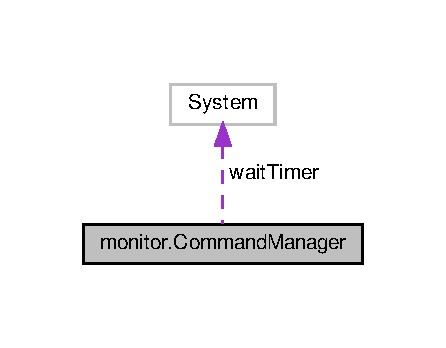
\includegraphics[width=214pt]{classmonitor_1_1_command_manager__coll__graph}
\end{center}
\end{figure}
\subsection*{Public Types}
\begin{DoxyCompactItemize}
\item 
enum \textbf{ Command\+Manager\+Status} \{ \textbf{ Command\+Manager\+Status.\+Answer\+Received}, 
\textbf{ Command\+Manager\+Status.\+Timeout}, 
\textbf{ Command\+Manager\+Status.\+Busy}
 \}\begin{DoxyCompactList}\small\item\em Available status when sending command \end{DoxyCompactList}
\end{DoxyCompactItemize}
\subsection*{Public Member Functions}
\begin{DoxyCompactItemize}
\item 
delegate void \textbf{ Command\+Received\+Event} (string msg, byte[$\,$] buffer)
\begin{DoxyCompactList}\small\item\em Callback for sending received data to upper level \end{DoxyCompactList}\item 
\textbf{ Command\+Manager} (\textbf{ Command\+Received\+Event} callback)
\begin{DoxyCompactList}\small\item\em Initializes a new instance of the T\+:monitor.\+Command\+Manager class. \end{DoxyCompactList}\item 
bool \textbf{ Open} (string hostname)
\begin{DoxyCompactList}\small\item\em Open the specified hostname server, using default port number. \end{DoxyCompactList}\item 
bool \textbf{ Open} (string hostname, int port)
\begin{DoxyCompactList}\small\item\em Open connection to server \char`\"{}host\char`\"{}, with port number \char`\"{}port\char`\"{} \end{DoxyCompactList}\item 
void \textbf{ Close} ()
\begin{DoxyCompactList}\small\item\em Close connection to server \end{DoxyCompactList}\item 
\textbf{ Command\+Manager\+Status} \textbf{ Send\+Command} (string cmd, out string answer, double timeout)
\begin{DoxyCompactList}\small\item\em Sends a command to T\+CP server \end{DoxyCompactList}\end{DoxyCompactItemize}
\subsection*{Public Attributes}
\begin{DoxyCompactItemize}
\item 
\textbf{ Command\+Received\+Event} \textbf{ command\+Received\+Event} = null
\end{DoxyCompactItemize}
\subsection*{Private Member Functions}
\begin{DoxyCompactItemize}
\item 
\textbf{ $\sim$\+Command\+Manager} ()
\begin{DoxyCompactList}\small\item\em Releases unmanaged resources and performs other cleanup operations before the T\+:monitor.\+Command\+Manager is reclaimed by garbage collection. \end{DoxyCompactList}\item 
void \textbf{ On\+Message\+Reception} (string message, byte[$\,$] buffer)
\begin{DoxyCompactList}\small\item\em Callback called by \doxyref{Client}{p.}{classmonitor_1_1_client} class after reception of new message \end{DoxyCompactList}\item 
void \textbf{ On\+Message\+Timeout} (object sender, System.\+Timers.\+Elapsed\+Event\+Args e)
\begin{DoxyCompactList}\small\item\em Callback called by stopwatch on timeout \end{DoxyCompactList}\end{DoxyCompactItemize}
\subsection*{Private Attributes}
\begin{DoxyCompactItemize}
\item 
System.\+Timers.\+Timer \textbf{ wait\+Timer} = new System.\+Timers.\+Timer()
\begin{DoxyCompactList}\small\item\em Timer for managing timeout \end{DoxyCompactList}\item 
Manual\+Reset\+Event \textbf{ wait\+Event} = new Manual\+Reset\+Event(false)
\item 
bool \textbf{ wait\+For\+Acknowledge} = false
\begin{DoxyCompactList}\small\item\em Flag to tell rogram to wait for an acknowledge from server \end{DoxyCompactList}\item 
string \textbf{ message\+Received} = null
\begin{DoxyCompactList}\small\item\em received message \end{DoxyCompactList}\item 
bool \textbf{ is\+Busy} = false
\begin{DoxyCompactList}\small\item\em flag indicating command manager is currently busy waiting an acknowledge \end{DoxyCompactList}\end{DoxyCompactItemize}


\subsection{Detailed Description}
Command Manager. Use for timeout managment during reception of data Used as intermediate layer between T\+CP client class (\doxyref{Client}{p.}{classmonitor_1_1_client}) and application level managment of command and answers 



Definition at line 31 of file Command\+Manager.\+cs.



\subsection{Member Enumeration Documentation}
\mbox{\label{classmonitor_1_1_command_manager_ac8ca53031468acc8be05c37586671a9b}} 
\index{monitor\+::\+Command\+Manager@{monitor\+::\+Command\+Manager}!Command\+Manager\+Status@{Command\+Manager\+Status}}
\index{Command\+Manager\+Status@{Command\+Manager\+Status}!monitor\+::\+Command\+Manager@{monitor\+::\+Command\+Manager}}
\subsubsection{Command\+Manager\+Status}
{\footnotesize\ttfamily enum \textbf{ monitor.\+Command\+Manager.\+Command\+Manager\+Status}\hspace{0.3cm}{\ttfamily [strong]}}



Available status when sending command 

\begin{DoxyEnumFields}{Enumerator}
\raisebox{\heightof{T}}[0pt][0pt]{\index{Answer\+Received@{Answer\+Received}!monitor\+::\+Command\+Manager@{monitor\+::\+Command\+Manager}}\index{monitor\+::\+Command\+Manager@{monitor\+::\+Command\+Manager}!Answer\+Received@{Answer\+Received}}}\mbox{\label{classmonitor_1_1_command_manager_ac8ca53031468acc8be05c37586671a9bae3e095863e3b99e11e8c18efb3901da3}} 
Answer\+Received&\\
\hline

\raisebox{\heightof{T}}[0pt][0pt]{\index{Timeout@{Timeout}!monitor\+::\+Command\+Manager@{monitor\+::\+Command\+Manager}}\index{monitor\+::\+Command\+Manager@{monitor\+::\+Command\+Manager}!Timeout@{Timeout}}}\mbox{\label{classmonitor_1_1_command_manager_ac8ca53031468acc8be05c37586671a9bac85a251cc457840f1e032f1b733e9398}} 
Timeout&\\
\hline

\raisebox{\heightof{T}}[0pt][0pt]{\index{Busy@{Busy}!monitor\+::\+Command\+Manager@{monitor\+::\+Command\+Manager}}\index{monitor\+::\+Command\+Manager@{monitor\+::\+Command\+Manager}!Busy@{Busy}}}\mbox{\label{classmonitor_1_1_command_manager_ac8ca53031468acc8be05c37586671a9bad8a942ef2b04672adfafef0ad817a407}} 
Busy&\\
\hline

\end{DoxyEnumFields}


Definition at line 63 of file Command\+Manager.\+cs.



\subsection{Constructor \& Destructor Documentation}
\mbox{\label{classmonitor_1_1_command_manager_ac2248c90d3a59bc2bf376cd876cece72}} 
\index{monitor\+::\+Command\+Manager@{monitor\+::\+Command\+Manager}!Command\+Manager@{Command\+Manager}}
\index{Command\+Manager@{Command\+Manager}!monitor\+::\+Command\+Manager@{monitor\+::\+Command\+Manager}}
\subsubsection{Command\+Manager()}
{\footnotesize\ttfamily monitor.\+Command\+Manager.\+Command\+Manager (\begin{DoxyParamCaption}\item[{\textbf{ Command\+Received\+Event}}]{callback }\end{DoxyParamCaption})}



Initializes a new instance of the T\+:monitor.\+Command\+Manager class. 


\begin{DoxyParams}{Parameters}
{\em callback} & Callback used when new message are received\\
\hline
\end{DoxyParams}


Definition at line 74 of file Command\+Manager.\+cs.

\mbox{\label{classmonitor_1_1_command_manager_ad2a8eb1139a5a25a6993887c55b3da4e}} 
\index{monitor\+::\+Command\+Manager@{monitor\+::\+Command\+Manager}!````~Command\+Manager@{$\sim$\+Command\+Manager}}
\index{````~Command\+Manager@{$\sim$\+Command\+Manager}!monitor\+::\+Command\+Manager@{monitor\+::\+Command\+Manager}}
\subsubsection{$\sim$\+Command\+Manager()}
{\footnotesize\ttfamily monitor.\+Command\+Manager.$\sim$\+Command\+Manager (\begin{DoxyParamCaption}{ }\end{DoxyParamCaption})\hspace{0.3cm}{\ttfamily [private]}}



Releases unmanaged resources and performs other cleanup operations before the T\+:monitor.\+Command\+Manager is reclaimed by garbage collection. 



Definition at line 86 of file Command\+Manager.\+cs.



\subsection{Member Function Documentation}
\mbox{\label{classmonitor_1_1_command_manager_ab28b0e5a2641391e655aaaaa05a1fdf6}} 
\index{monitor\+::\+Command\+Manager@{monitor\+::\+Command\+Manager}!Close@{Close}}
\index{Close@{Close}!monitor\+::\+Command\+Manager@{monitor\+::\+Command\+Manager}}
\subsubsection{Close()}
{\footnotesize\ttfamily void monitor.\+Command\+Manager.\+Close (\begin{DoxyParamCaption}{ }\end{DoxyParamCaption})}



Close connection to server 



Definition at line 115 of file Command\+Manager.\+cs.

\mbox{\label{classmonitor_1_1_command_manager_a5afd16036cc3d0e69554f69dacad0bcc}} 
\index{monitor\+::\+Command\+Manager@{monitor\+::\+Command\+Manager}!Command\+Received\+Event@{Command\+Received\+Event}}
\index{Command\+Received\+Event@{Command\+Received\+Event}!monitor\+::\+Command\+Manager@{monitor\+::\+Command\+Manager}}
\subsubsection{Command\+Received\+Event()}
{\footnotesize\ttfamily delegate void monitor.\+Command\+Manager.\+Command\+Received\+Event (\begin{DoxyParamCaption}\item[{string}]{msg,  }\item[{byte [$\,$]}]{buffer }\end{DoxyParamCaption})}



Callback for sending received data to upper level 

\mbox{\label{classmonitor_1_1_command_manager_a92e5d42afb61f29d9a4746b4446c2a65}} 
\index{monitor\+::\+Command\+Manager@{monitor\+::\+Command\+Manager}!On\+Message\+Reception@{On\+Message\+Reception}}
\index{On\+Message\+Reception@{On\+Message\+Reception}!monitor\+::\+Command\+Manager@{monitor\+::\+Command\+Manager}}
\subsubsection{On\+Message\+Reception()}
{\footnotesize\ttfamily void monitor.\+Command\+Manager.\+On\+Message\+Reception (\begin{DoxyParamCaption}\item[{string}]{message,  }\item[{byte [$\,$]}]{buffer }\end{DoxyParamCaption})\hspace{0.3cm}{\ttfamily [private]}}



Callback called by \doxyref{Client}{p.}{classmonitor_1_1_client} class after reception of new message 


\begin{DoxyParams}{Parameters}
{\em message} & Message received from server\\
\hline
{\em buffer} & Raw buffer reived from server\\
\hline
\end{DoxyParams}


Definition at line 125 of file Command\+Manager.\+cs.

\mbox{\label{classmonitor_1_1_command_manager_a2f91bb775ba25855be007886b994a5df}} 
\index{monitor\+::\+Command\+Manager@{monitor\+::\+Command\+Manager}!On\+Message\+Timeout@{On\+Message\+Timeout}}
\index{On\+Message\+Timeout@{On\+Message\+Timeout}!monitor\+::\+Command\+Manager@{monitor\+::\+Command\+Manager}}
\subsubsection{On\+Message\+Timeout()}
{\footnotesize\ttfamily void monitor.\+Command\+Manager.\+On\+Message\+Timeout (\begin{DoxyParamCaption}\item[{object}]{sender,  }\item[{System.\+Timers.\+Elapsed\+Event\+Args}]{e }\end{DoxyParamCaption})\hspace{0.3cm}{\ttfamily [private]}}



Callback called by stopwatch on timeout 


\begin{DoxyParams}{Parameters}
{\em sender} & Sender object\\
\hline
{\em e} & Information on elapsed condition\\
\hline
\end{DoxyParams}


Definition at line 156 of file Command\+Manager.\+cs.

\mbox{\label{classmonitor_1_1_command_manager_a7329cbf8008bcb8a0280aa7ffa6aa43c}} 
\index{monitor\+::\+Command\+Manager@{monitor\+::\+Command\+Manager}!Open@{Open}}
\index{Open@{Open}!monitor\+::\+Command\+Manager@{monitor\+::\+Command\+Manager}}
\subsubsection{Open()\hspace{0.1cm}{\footnotesize\ttfamily [1/2]}}
{\footnotesize\ttfamily bool monitor.\+Command\+Manager.\+Open (\begin{DoxyParamCaption}\item[{string}]{hostname }\end{DoxyParamCaption})}



Open the specified hostname server, using default port number. 

\begin{DoxyReturn}{Returns}
true if connection succeded, false otherwise
\end{DoxyReturn}

\begin{DoxyParams}{Parameters}
{\em hostname} & Hostname to connect to\\
\hline
\end{DoxyParams}


Definition at line 96 of file Command\+Manager.\+cs.

\mbox{\label{classmonitor_1_1_command_manager_a0a0054ee87d293577fa39af1fcd5ffee}} 
\index{monitor\+::\+Command\+Manager@{monitor\+::\+Command\+Manager}!Open@{Open}}
\index{Open@{Open}!monitor\+::\+Command\+Manager@{monitor\+::\+Command\+Manager}}
\subsubsection{Open()\hspace{0.1cm}{\footnotesize\ttfamily [2/2]}}
{\footnotesize\ttfamily bool monitor.\+Command\+Manager.\+Open (\begin{DoxyParamCaption}\item[{string}]{hostname,  }\item[{int}]{port }\end{DoxyParamCaption})}



Open connection to server \char`\"{}host\char`\"{}, with port number \char`\"{}port\char`\"{} 

\begin{DoxyReturn}{Returns}
true if connection succeded, false otherwise
\end{DoxyReturn}

\begin{DoxyParams}{Parameters}
{\em hostname} & Hostname to connect to\\
\hline
{\em port} & Port number for connection\\
\hline
\end{DoxyParams}


Definition at line 107 of file Command\+Manager.\+cs.

\mbox{\label{classmonitor_1_1_command_manager_a3cd1f2303e47e5148fd3e927a7957363}} 
\index{monitor\+::\+Command\+Manager@{monitor\+::\+Command\+Manager}!Send\+Command@{Send\+Command}}
\index{Send\+Command@{Send\+Command}!monitor\+::\+Command\+Manager@{monitor\+::\+Command\+Manager}}
\subsubsection{Send\+Command()}
{\footnotesize\ttfamily \textbf{ Command\+Manager\+Status} monitor.\+Command\+Manager.\+Send\+Command (\begin{DoxyParamCaption}\item[{string}]{cmd,  }\item[{out string}]{answer,  }\item[{double}]{timeout }\end{DoxyParamCaption})}



Sends a command to T\+CP server 

\begin{DoxyReturn}{Returns}
status that is part of Command\+Manager\+Status enumerate
\end{DoxyReturn}

\begin{DoxyParams}{Parameters}
{\em cmd} & Command message to send to server\\
\hline
{\em answer} & Answer from server, in case of acknowledge\\
\hline
{\em timeout} & Timeout (ms) waiting an acknowledge, 0 if no acknowledge needed\\
\hline
\end{DoxyParams}


Definition at line 171 of file Command\+Manager.\+cs.



\subsection{Member Data Documentation}
\mbox{\label{classmonitor_1_1_command_manager_ab90d68a3d3a9b3935fa9f1a57e8dabfa}} 
\index{monitor\+::\+Command\+Manager@{monitor\+::\+Command\+Manager}!command\+Received\+Event@{command\+Received\+Event}}
\index{command\+Received\+Event@{command\+Received\+Event}!monitor\+::\+Command\+Manager@{monitor\+::\+Command\+Manager}}
\subsubsection{command\+Received\+Event}
{\footnotesize\ttfamily \textbf{ Command\+Received\+Event} monitor.\+Command\+Manager.\+command\+Received\+Event = null}



Definition at line 37 of file Command\+Manager.\+cs.

\mbox{\label{classmonitor_1_1_command_manager_aea039cd0f99f5193c307b805077669db}} 
\index{monitor\+::\+Command\+Manager@{monitor\+::\+Command\+Manager}!is\+Busy@{is\+Busy}}
\index{is\+Busy@{is\+Busy}!monitor\+::\+Command\+Manager@{monitor\+::\+Command\+Manager}}
\subsubsection{is\+Busy}
{\footnotesize\ttfamily bool monitor.\+Command\+Manager.\+is\+Busy = false\hspace{0.3cm}{\ttfamily [private]}}



flag indicating command manager is currently busy waiting an acknowledge 



Definition at line 58 of file Command\+Manager.\+cs.

\mbox{\label{classmonitor_1_1_command_manager_aa610e72e8f23f0d26388f204c848ed57}} 
\index{monitor\+::\+Command\+Manager@{monitor\+::\+Command\+Manager}!message\+Received@{message\+Received}}
\index{message\+Received@{message\+Received}!monitor\+::\+Command\+Manager@{monitor\+::\+Command\+Manager}}
\subsubsection{message\+Received}
{\footnotesize\ttfamily string monitor.\+Command\+Manager.\+message\+Received = null\hspace{0.3cm}{\ttfamily [private]}}



received message 



Definition at line 53 of file Command\+Manager.\+cs.

\mbox{\label{classmonitor_1_1_command_manager_a0d27eb1a38efb01559f14a707ff86447}} 
\index{monitor\+::\+Command\+Manager@{monitor\+::\+Command\+Manager}!wait\+Event@{wait\+Event}}
\index{wait\+Event@{wait\+Event}!monitor\+::\+Command\+Manager@{monitor\+::\+Command\+Manager}}
\subsubsection{wait\+Event}
{\footnotesize\ttfamily Manual\+Reset\+Event monitor.\+Command\+Manager.\+wait\+Event = new Manual\+Reset\+Event(false)\hspace{0.3cm}{\ttfamily [private]}}



Definition at line 43 of file Command\+Manager.\+cs.

\mbox{\label{classmonitor_1_1_command_manager_a39c2c03f93b309e65a45ac91c6eb39bd}} 
\index{monitor\+::\+Command\+Manager@{monitor\+::\+Command\+Manager}!wait\+For\+Acknowledge@{wait\+For\+Acknowledge}}
\index{wait\+For\+Acknowledge@{wait\+For\+Acknowledge}!monitor\+::\+Command\+Manager@{monitor\+::\+Command\+Manager}}
\subsubsection{wait\+For\+Acknowledge}
{\footnotesize\ttfamily bool monitor.\+Command\+Manager.\+wait\+For\+Acknowledge = false\hspace{0.3cm}{\ttfamily [private]}}



Flag to tell rogram to wait for an acknowledge from server 



Definition at line 48 of file Command\+Manager.\+cs.

\mbox{\label{classmonitor_1_1_command_manager_a07639cd39445a379667a2450e78001b0}} 
\index{monitor\+::\+Command\+Manager@{monitor\+::\+Command\+Manager}!wait\+Timer@{wait\+Timer}}
\index{wait\+Timer@{wait\+Timer}!monitor\+::\+Command\+Manager@{monitor\+::\+Command\+Manager}}
\subsubsection{wait\+Timer}
{\footnotesize\ttfamily System.\+Timers.\+Timer monitor.\+Command\+Manager.\+wait\+Timer = new System.\+Timers.\+Timer()\hspace{0.3cm}{\ttfamily [private]}}



Timer for managing timeout 



Definition at line 42 of file Command\+Manager.\+cs.



The documentation for this class was generated from the following file\+:\begin{DoxyCompactItemize}
\item 
\textbf{ Command\+Manager.\+cs}\end{DoxyCompactItemize}

\section{monitor.\+Destijl\+Command\+List Class Reference}
\label{classmonitor_1_1_destijl_command_list}\index{monitor.\+Destijl\+Command\+List@{monitor.\+Destijl\+Command\+List}}
\subsection*{Public Attributes}
\begin{DoxyCompactItemize}
\item 
const string \textbf{ Header\+Mts\+Com\+Dmb} = \char`\"{}C\+OM\char`\"{}
\item 
const string \textbf{ Header\+Mts\+Dmb\+Order} = \char`\"{}D\+MB\char`\"{}
\item 
const string \textbf{ Header\+Mts\+Camera} = \char`\"{}C\+AM\char`\"{}
\item 
const string \textbf{ Header\+Mts\+Message} = \char`\"{}M\+SG\char`\"{}
\item 
const string \textbf{ Data\+Com\+Open} = \char`\"{}o\char`\"{}
\item 
const string \textbf{ Data\+Com\+Close} = \char`\"{}C\char`\"{}
\item 
const string \textbf{ Data\+Cam\+Open} = \char`\"{}A\char`\"{}
\item 
const string \textbf{ Data\+Cam\+Close} = \char`\"{}I\char`\"{}
\item 
const string \textbf{ Data\+Cam\+Ask\+Arena} = \char`\"{}y\char`\"{}
\item 
const string \textbf{ Data\+Cam\+Arena\+Confirm} = \char`\"{}x\char`\"{}
\item 
const string \textbf{ Data\+Cam\+Infirm} = \char`\"{}z\char`\"{}
\item 
const string \textbf{ Data\+Cam\+Compute\+Position} = \char`\"{}p\char`\"{}
\item 
const string \textbf{ Data\+Cam\+Stop\+Compute\+Position} = \char`\"{}s\char`\"{}
\item 
const string \textbf{ Header\+Stm\+Ack} = \char`\"{}A\+CK\char`\"{}
\item 
const string \textbf{ Header\+Stm\+No\+Ack} = \char`\"{}N\+AK\char`\"{}
\item 
const string \textbf{ Header\+Stm\+Lost\+Dmb} = \char`\"{}L\+CD\char`\"{}
\item 
const string \textbf{ Header\+Stm\+Image} = \char`\"{}I\+MG\char`\"{}
\item 
const string \textbf{ Header\+Stm\+Pos} = \char`\"{}P\+OS\char`\"{}
\item 
const string \textbf{ Header\+Stm\+Mes} = \char`\"{}M\+SG\char`\"{}
\item 
const string \textbf{ Header\+Stm\+Bat} = \char`\"{}B\+AT\char`\"{}
\end{DoxyCompactItemize}


\subsection{Detailed Description}


Definition at line 5 of file Destijl\+Command\+Manager.\+cs.



\subsection{Member Data Documentation}
\mbox{\label{classmonitor_1_1_destijl_command_list_ad31b6758839a4c3b1b6ec4c71635e631}} 
\index{monitor\+::\+Destijl\+Command\+List@{monitor\+::\+Destijl\+Command\+List}!Data\+Cam\+Arena\+Confirm@{Data\+Cam\+Arena\+Confirm}}
\index{Data\+Cam\+Arena\+Confirm@{Data\+Cam\+Arena\+Confirm}!monitor\+::\+Destijl\+Command\+List@{monitor\+::\+Destijl\+Command\+List}}
\subsubsection{Data\+Cam\+Arena\+Confirm}
{\footnotesize\ttfamily const string monitor.\+Destijl\+Command\+List.\+Data\+Cam\+Arena\+Confirm = \char`\"{}x\char`\"{}}



Definition at line 18 of file Destijl\+Command\+Manager.\+cs.

\mbox{\label{classmonitor_1_1_destijl_command_list_aaaf85677671db1ef84fe67b2eb954f29}} 
\index{monitor\+::\+Destijl\+Command\+List@{monitor\+::\+Destijl\+Command\+List}!Data\+Cam\+Ask\+Arena@{Data\+Cam\+Ask\+Arena}}
\index{Data\+Cam\+Ask\+Arena@{Data\+Cam\+Ask\+Arena}!monitor\+::\+Destijl\+Command\+List@{monitor\+::\+Destijl\+Command\+List}}
\subsubsection{Data\+Cam\+Ask\+Arena}
{\footnotesize\ttfamily const string monitor.\+Destijl\+Command\+List.\+Data\+Cam\+Ask\+Arena = \char`\"{}y\char`\"{}}



Definition at line 17 of file Destijl\+Command\+Manager.\+cs.

\mbox{\label{classmonitor_1_1_destijl_command_list_a6f578f9d52dd2b50370177a5c03a2af7}} 
\index{monitor\+::\+Destijl\+Command\+List@{monitor\+::\+Destijl\+Command\+List}!Data\+Cam\+Close@{Data\+Cam\+Close}}
\index{Data\+Cam\+Close@{Data\+Cam\+Close}!monitor\+::\+Destijl\+Command\+List@{monitor\+::\+Destijl\+Command\+List}}
\subsubsection{Data\+Cam\+Close}
{\footnotesize\ttfamily const string monitor.\+Destijl\+Command\+List.\+Data\+Cam\+Close = \char`\"{}I\char`\"{}}



Definition at line 16 of file Destijl\+Command\+Manager.\+cs.

\mbox{\label{classmonitor_1_1_destijl_command_list_ab114adce60b63976d8304f2ad11b317a}} 
\index{monitor\+::\+Destijl\+Command\+List@{monitor\+::\+Destijl\+Command\+List}!Data\+Cam\+Compute\+Position@{Data\+Cam\+Compute\+Position}}
\index{Data\+Cam\+Compute\+Position@{Data\+Cam\+Compute\+Position}!monitor\+::\+Destijl\+Command\+List@{monitor\+::\+Destijl\+Command\+List}}
\subsubsection{Data\+Cam\+Compute\+Position}
{\footnotesize\ttfamily const string monitor.\+Destijl\+Command\+List.\+Data\+Cam\+Compute\+Position = \char`\"{}p\char`\"{}}



Definition at line 20 of file Destijl\+Command\+Manager.\+cs.

\mbox{\label{classmonitor_1_1_destijl_command_list_ad3985694a06148f2014cb346e8891cba}} 
\index{monitor\+::\+Destijl\+Command\+List@{monitor\+::\+Destijl\+Command\+List}!Data\+Cam\+Infirm@{Data\+Cam\+Infirm}}
\index{Data\+Cam\+Infirm@{Data\+Cam\+Infirm}!monitor\+::\+Destijl\+Command\+List@{monitor\+::\+Destijl\+Command\+List}}
\subsubsection{Data\+Cam\+Infirm}
{\footnotesize\ttfamily const string monitor.\+Destijl\+Command\+List.\+Data\+Cam\+Infirm = \char`\"{}z\char`\"{}}



Definition at line 19 of file Destijl\+Command\+Manager.\+cs.

\mbox{\label{classmonitor_1_1_destijl_command_list_a6380d1518931373bd0dfb84f888942e0}} 
\index{monitor\+::\+Destijl\+Command\+List@{monitor\+::\+Destijl\+Command\+List}!Data\+Cam\+Open@{Data\+Cam\+Open}}
\index{Data\+Cam\+Open@{Data\+Cam\+Open}!monitor\+::\+Destijl\+Command\+List@{monitor\+::\+Destijl\+Command\+List}}
\subsubsection{Data\+Cam\+Open}
{\footnotesize\ttfamily const string monitor.\+Destijl\+Command\+List.\+Data\+Cam\+Open = \char`\"{}A\char`\"{}}



Definition at line 15 of file Destijl\+Command\+Manager.\+cs.

\mbox{\label{classmonitor_1_1_destijl_command_list_ad09dd921c6c8cf8c7d90a2c0a05d4056}} 
\index{monitor\+::\+Destijl\+Command\+List@{monitor\+::\+Destijl\+Command\+List}!Data\+Cam\+Stop\+Compute\+Position@{Data\+Cam\+Stop\+Compute\+Position}}
\index{Data\+Cam\+Stop\+Compute\+Position@{Data\+Cam\+Stop\+Compute\+Position}!monitor\+::\+Destijl\+Command\+List@{monitor\+::\+Destijl\+Command\+List}}
\subsubsection{Data\+Cam\+Stop\+Compute\+Position}
{\footnotesize\ttfamily const string monitor.\+Destijl\+Command\+List.\+Data\+Cam\+Stop\+Compute\+Position = \char`\"{}s\char`\"{}}



Definition at line 21 of file Destijl\+Command\+Manager.\+cs.

\mbox{\label{classmonitor_1_1_destijl_command_list_ad97cbe948c71a4dc3fa95afbf9ca26d8}} 
\index{monitor\+::\+Destijl\+Command\+List@{monitor\+::\+Destijl\+Command\+List}!Data\+Com\+Close@{Data\+Com\+Close}}
\index{Data\+Com\+Close@{Data\+Com\+Close}!monitor\+::\+Destijl\+Command\+List@{monitor\+::\+Destijl\+Command\+List}}
\subsubsection{Data\+Com\+Close}
{\footnotesize\ttfamily const string monitor.\+Destijl\+Command\+List.\+Data\+Com\+Close = \char`\"{}C\char`\"{}}



Definition at line 13 of file Destijl\+Command\+Manager.\+cs.

\mbox{\label{classmonitor_1_1_destijl_command_list_a1bcde55da429bcf2c04ed6d0621e496f}} 
\index{monitor\+::\+Destijl\+Command\+List@{monitor\+::\+Destijl\+Command\+List}!Data\+Com\+Open@{Data\+Com\+Open}}
\index{Data\+Com\+Open@{Data\+Com\+Open}!monitor\+::\+Destijl\+Command\+List@{monitor\+::\+Destijl\+Command\+List}}
\subsubsection{Data\+Com\+Open}
{\footnotesize\ttfamily const string monitor.\+Destijl\+Command\+List.\+Data\+Com\+Open = \char`\"{}o\char`\"{}}



Definition at line 12 of file Destijl\+Command\+Manager.\+cs.

\mbox{\label{classmonitor_1_1_destijl_command_list_af570b0e8d14920402ce979778225ed68}} 
\index{monitor\+::\+Destijl\+Command\+List@{monitor\+::\+Destijl\+Command\+List}!Header\+Mts\+Camera@{Header\+Mts\+Camera}}
\index{Header\+Mts\+Camera@{Header\+Mts\+Camera}!monitor\+::\+Destijl\+Command\+List@{monitor\+::\+Destijl\+Command\+List}}
\subsubsection{Header\+Mts\+Camera}
{\footnotesize\ttfamily const string monitor.\+Destijl\+Command\+List.\+Header\+Mts\+Camera = \char`\"{}C\+AM\char`\"{}}



Definition at line 9 of file Destijl\+Command\+Manager.\+cs.

\mbox{\label{classmonitor_1_1_destijl_command_list_aa9fe4e71b7faec183ab64f4cf6ecd395}} 
\index{monitor\+::\+Destijl\+Command\+List@{monitor\+::\+Destijl\+Command\+List}!Header\+Mts\+Com\+Dmb@{Header\+Mts\+Com\+Dmb}}
\index{Header\+Mts\+Com\+Dmb@{Header\+Mts\+Com\+Dmb}!monitor\+::\+Destijl\+Command\+List@{monitor\+::\+Destijl\+Command\+List}}
\subsubsection{Header\+Mts\+Com\+Dmb}
{\footnotesize\ttfamily const string monitor.\+Destijl\+Command\+List.\+Header\+Mts\+Com\+Dmb = \char`\"{}C\+OM\char`\"{}}



Definition at line 7 of file Destijl\+Command\+Manager.\+cs.

\mbox{\label{classmonitor_1_1_destijl_command_list_adbcf7adab9f5e8ead971affbbc64178b}} 
\index{monitor\+::\+Destijl\+Command\+List@{monitor\+::\+Destijl\+Command\+List}!Header\+Mts\+Dmb\+Order@{Header\+Mts\+Dmb\+Order}}
\index{Header\+Mts\+Dmb\+Order@{Header\+Mts\+Dmb\+Order}!monitor\+::\+Destijl\+Command\+List@{monitor\+::\+Destijl\+Command\+List}}
\subsubsection{Header\+Mts\+Dmb\+Order}
{\footnotesize\ttfamily const string monitor.\+Destijl\+Command\+List.\+Header\+Mts\+Dmb\+Order = \char`\"{}D\+MB\char`\"{}}



Definition at line 8 of file Destijl\+Command\+Manager.\+cs.

\mbox{\label{classmonitor_1_1_destijl_command_list_acb283f1da96d8d522e3b28ca35187acd}} 
\index{monitor\+::\+Destijl\+Command\+List@{monitor\+::\+Destijl\+Command\+List}!Header\+Mts\+Message@{Header\+Mts\+Message}}
\index{Header\+Mts\+Message@{Header\+Mts\+Message}!monitor\+::\+Destijl\+Command\+List@{monitor\+::\+Destijl\+Command\+List}}
\subsubsection{Header\+Mts\+Message}
{\footnotesize\ttfamily const string monitor.\+Destijl\+Command\+List.\+Header\+Mts\+Message = \char`\"{}M\+SG\char`\"{}}



Definition at line 10 of file Destijl\+Command\+Manager.\+cs.

\mbox{\label{classmonitor_1_1_destijl_command_list_af494d7e1bddee8184873dc380a3066ba}} 
\index{monitor\+::\+Destijl\+Command\+List@{monitor\+::\+Destijl\+Command\+List}!Header\+Stm\+Ack@{Header\+Stm\+Ack}}
\index{Header\+Stm\+Ack@{Header\+Stm\+Ack}!monitor\+::\+Destijl\+Command\+List@{monitor\+::\+Destijl\+Command\+List}}
\subsubsection{Header\+Stm\+Ack}
{\footnotesize\ttfamily const string monitor.\+Destijl\+Command\+List.\+Header\+Stm\+Ack = \char`\"{}A\+CK\char`\"{}}



Definition at line 23 of file Destijl\+Command\+Manager.\+cs.

\mbox{\label{classmonitor_1_1_destijl_command_list_a88de91fa6abdc122245ceb26fc21fd33}} 
\index{monitor\+::\+Destijl\+Command\+List@{monitor\+::\+Destijl\+Command\+List}!Header\+Stm\+Bat@{Header\+Stm\+Bat}}
\index{Header\+Stm\+Bat@{Header\+Stm\+Bat}!monitor\+::\+Destijl\+Command\+List@{monitor\+::\+Destijl\+Command\+List}}
\subsubsection{Header\+Stm\+Bat}
{\footnotesize\ttfamily const string monitor.\+Destijl\+Command\+List.\+Header\+Stm\+Bat = \char`\"{}B\+AT\char`\"{}}



Definition at line 29 of file Destijl\+Command\+Manager.\+cs.

\mbox{\label{classmonitor_1_1_destijl_command_list_ae3ee8e0ecbb79faec9d24095d72cfbde}} 
\index{monitor\+::\+Destijl\+Command\+List@{monitor\+::\+Destijl\+Command\+List}!Header\+Stm\+Image@{Header\+Stm\+Image}}
\index{Header\+Stm\+Image@{Header\+Stm\+Image}!monitor\+::\+Destijl\+Command\+List@{monitor\+::\+Destijl\+Command\+List}}
\subsubsection{Header\+Stm\+Image}
{\footnotesize\ttfamily const string monitor.\+Destijl\+Command\+List.\+Header\+Stm\+Image = \char`\"{}I\+MG\char`\"{}}



Definition at line 26 of file Destijl\+Command\+Manager.\+cs.

\mbox{\label{classmonitor_1_1_destijl_command_list_a54e9ebd5e8f34ac596b84b56bb2403f7}} 
\index{monitor\+::\+Destijl\+Command\+List@{monitor\+::\+Destijl\+Command\+List}!Header\+Stm\+Lost\+Dmb@{Header\+Stm\+Lost\+Dmb}}
\index{Header\+Stm\+Lost\+Dmb@{Header\+Stm\+Lost\+Dmb}!monitor\+::\+Destijl\+Command\+List@{monitor\+::\+Destijl\+Command\+List}}
\subsubsection{Header\+Stm\+Lost\+Dmb}
{\footnotesize\ttfamily const string monitor.\+Destijl\+Command\+List.\+Header\+Stm\+Lost\+Dmb = \char`\"{}L\+CD\char`\"{}}



Definition at line 25 of file Destijl\+Command\+Manager.\+cs.

\mbox{\label{classmonitor_1_1_destijl_command_list_ad1fa4557b2d44dd888d8640f374c9f04}} 
\index{monitor\+::\+Destijl\+Command\+List@{monitor\+::\+Destijl\+Command\+List}!Header\+Stm\+Mes@{Header\+Stm\+Mes}}
\index{Header\+Stm\+Mes@{Header\+Stm\+Mes}!monitor\+::\+Destijl\+Command\+List@{monitor\+::\+Destijl\+Command\+List}}
\subsubsection{Header\+Stm\+Mes}
{\footnotesize\ttfamily const string monitor.\+Destijl\+Command\+List.\+Header\+Stm\+Mes = \char`\"{}M\+SG\char`\"{}}



Definition at line 28 of file Destijl\+Command\+Manager.\+cs.

\mbox{\label{classmonitor_1_1_destijl_command_list_ae3dc86c7e90bba409317e63cf1c85a39}} 
\index{monitor\+::\+Destijl\+Command\+List@{monitor\+::\+Destijl\+Command\+List}!Header\+Stm\+No\+Ack@{Header\+Stm\+No\+Ack}}
\index{Header\+Stm\+No\+Ack@{Header\+Stm\+No\+Ack}!monitor\+::\+Destijl\+Command\+List@{monitor\+::\+Destijl\+Command\+List}}
\subsubsection{Header\+Stm\+No\+Ack}
{\footnotesize\ttfamily const string monitor.\+Destijl\+Command\+List.\+Header\+Stm\+No\+Ack = \char`\"{}N\+AK\char`\"{}}



Definition at line 24 of file Destijl\+Command\+Manager.\+cs.

\mbox{\label{classmonitor_1_1_destijl_command_list_abf99a718161a5a9017d7011cea429ec0}} 
\index{monitor\+::\+Destijl\+Command\+List@{monitor\+::\+Destijl\+Command\+List}!Header\+Stm\+Pos@{Header\+Stm\+Pos}}
\index{Header\+Stm\+Pos@{Header\+Stm\+Pos}!monitor\+::\+Destijl\+Command\+List@{monitor\+::\+Destijl\+Command\+List}}
\subsubsection{Header\+Stm\+Pos}
{\footnotesize\ttfamily const string monitor.\+Destijl\+Command\+List.\+Header\+Stm\+Pos = \char`\"{}P\+OS\char`\"{}}



Definition at line 27 of file Destijl\+Command\+Manager.\+cs.



The documentation for this class was generated from the following file\+:\begin{DoxyCompactItemize}
\item 
\textbf{ Destijl\+Command\+Manager.\+cs}\end{DoxyCompactItemize}

\section{monitor.\+Destijl\+Command\+Manager Class Reference}
\label{classmonitor_1_1_destijl_command_manager}\index{monitor.\+Destijl\+Command\+Manager@{monitor.\+Destijl\+Command\+Manager}}


Collaboration diagram for monitor.\+Destijl\+Command\+Manager\+:
\nopagebreak
\begin{figure}[H]
\begin{center}
\leavevmode
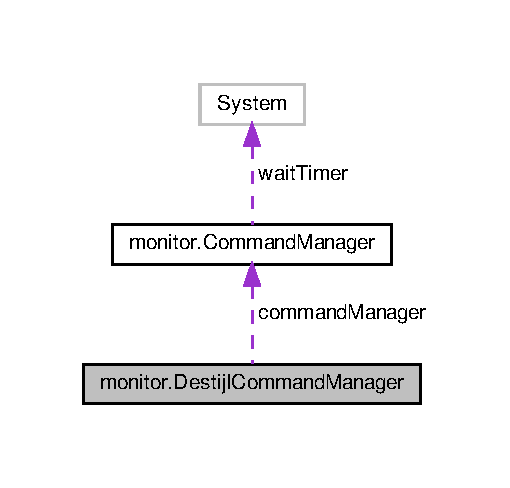
\includegraphics[width=245pt]{classmonitor_1_1_destijl_command_manager__coll__graph}
\end{center}
\end{figure}
\subsection*{Public Types}
\begin{DoxyCompactItemize}
\item 
enum \textbf{ Command\+Status} \{ \newline
\textbf{ Command\+Status.\+Success}, 
\textbf{ Command\+Status.\+Rejected}, 
\textbf{ Command\+Status.\+Invalid\+Answer}, 
\textbf{ Command\+Status.\+Busy}, 
\newline
\textbf{ Command\+Status.\+Communication\+Lost\+With\+Robot}, 
\textbf{ Command\+Status.\+Communication\+Lost\+With\+Server}
 \}
\end{DoxyCompactItemize}
\subsection*{Public Member Functions}
\begin{DoxyCompactItemize}
\item 
delegate void \textbf{ Command\+Received\+Event} (string header, string data, byte[$\,$] buffer)
\item 
\textbf{ Destijl\+Command\+Manager} (\textbf{ Command\+Received\+Event} callback)
\item 
bool \textbf{ Open} (string hostname)
\item 
bool \textbf{ Open} (string hostname, int port)
\item 
void \textbf{ Close} ()
\item 
\textbf{ Command\+Status} \textbf{ Robot\+Open\+Com} ()
\item 
\textbf{ Command\+Status} \textbf{ Robot\+Close\+Com} ()
\item 
\textbf{ Command\+Status} \textbf{ Robot\+Ping} ()
\item 
\textbf{ Command\+Status} \textbf{ Robot\+Reset} ()
\item 
\textbf{ Command\+Status} \textbf{ Robot\+Start\+With\+Watchdog} ()
\item 
\textbf{ Command\+Status} \textbf{ Robot\+Start\+Without\+Watchdog} ()
\item 
\textbf{ Command\+Status} \textbf{ Robot\+Move} (int distance)
\item 
\textbf{ Command\+Status} \textbf{ Robot\+Turn} (int angle)
\item 
\textbf{ Command\+Status} \textbf{ Robot\+Get\+Battery} ()
\item 
\textbf{ Command\+Status} \textbf{ Robot\+Get\+Version} (out string version)
\item 
\textbf{ Command\+Status} \textbf{ Robot\+Power\+Off} ()
\item 
\textbf{ Command\+Status} \textbf{ Camera\+Open} ()
\item 
\textbf{ Command\+Status} \textbf{ Camera\+Close} ()
\item 
\textbf{ Command\+Status} \textbf{ Camera\+Ask\+Arena} ()
\item 
\textbf{ Command\+Status} \textbf{ Camera\+Arena\+Confirm} ()
\item 
\textbf{ Command\+Status} \textbf{ Camera\+Arena\+Infirm} ()
\item 
\textbf{ Command\+Status} \textbf{ Camera\+Compute\+Position} ()
\item 
\textbf{ Command\+Status} \textbf{ Camera\+Stop\+Compute\+Position} ()
\end{DoxyCompactItemize}
\subsection*{Public Attributes}
\begin{DoxyCompactItemize}
\item 
\textbf{ Command\+Received\+Event} \textbf{ command\+Received\+Event} = null
\item 
double \textbf{ timeout} = 100
\end{DoxyCompactItemize}
\subsection*{Private Member Functions}
\begin{DoxyCompactItemize}
\item 
\textbf{ $\sim$\+Destijl\+Command\+Manager} ()
\item 
void \textbf{ On\+Command\+Received} (string msg, byte[$\,$] buffer)
\item 
string \textbf{ Create\+Command} (string header, string data)
\item 
void \textbf{ Split\+Command} (string cmd, out string header, out string data)
\item 
\textbf{ Command\+Status} \textbf{ Decode\+Status} (\textbf{ Command\+Manager.\+Command\+Manager\+Status} local\+Status, string answer)
\end{DoxyCompactItemize}
\subsection*{Private Attributes}
\begin{DoxyCompactItemize}
\item 
\textbf{ Command\+Manager} \textbf{ command\+Manager} = null
\item 
string \textbf{ received\+Header} = null
\item 
string \textbf{ received\+Data} = null
\end{DoxyCompactItemize}


\subsection{Detailed Description}


Definition at line 46 of file Destijl\+Command\+Manager.\+cs.



\subsection{Member Enumeration Documentation}
\mbox{\label{classmonitor_1_1_destijl_command_manager_a9cb23e7493a32872ac808f3b63200fb0}} 
\index{monitor\+::\+Destijl\+Command\+Manager@{monitor\+::\+Destijl\+Command\+Manager}!Command\+Status@{Command\+Status}}
\index{Command\+Status@{Command\+Status}!monitor\+::\+Destijl\+Command\+Manager@{monitor\+::\+Destijl\+Command\+Manager}}
\subsubsection{Command\+Status}
{\footnotesize\ttfamily enum \textbf{ monitor.\+Destijl\+Command\+Manager.\+Command\+Status}\hspace{0.3cm}{\ttfamily [strong]}}

\begin{DoxyEnumFields}{Enumerator}
\raisebox{\heightof{T}}[0pt][0pt]{\index{Success@{Success}!monitor\+::\+Destijl\+Command\+Manager@{monitor\+::\+Destijl\+Command\+Manager}}\index{monitor\+::\+Destijl\+Command\+Manager@{monitor\+::\+Destijl\+Command\+Manager}!Success@{Success}}}\mbox{\label{classmonitor_1_1_destijl_command_manager_a9cb23e7493a32872ac808f3b63200fb0a505a83f220c02df2f85c3810cd9ceb38}} 
Success&\\
\hline

\raisebox{\heightof{T}}[0pt][0pt]{\index{Rejected@{Rejected}!monitor\+::\+Destijl\+Command\+Manager@{monitor\+::\+Destijl\+Command\+Manager}}\index{monitor\+::\+Destijl\+Command\+Manager@{monitor\+::\+Destijl\+Command\+Manager}!Rejected@{Rejected}}}\mbox{\label{classmonitor_1_1_destijl_command_manager_a9cb23e7493a32872ac808f3b63200fb0ad37b1f6c0512e2118cee17fea015b699}} 
Rejected&\\
\hline

\raisebox{\heightof{T}}[0pt][0pt]{\index{Invalid\+Answer@{Invalid\+Answer}!monitor\+::\+Destijl\+Command\+Manager@{monitor\+::\+Destijl\+Command\+Manager}}\index{monitor\+::\+Destijl\+Command\+Manager@{monitor\+::\+Destijl\+Command\+Manager}!Invalid\+Answer@{Invalid\+Answer}}}\mbox{\label{classmonitor_1_1_destijl_command_manager_a9cb23e7493a32872ac808f3b63200fb0ad410f0b6f9dc2f2b271f9cf2fc78eb34}} 
Invalid\+Answer&\\
\hline

\raisebox{\heightof{T}}[0pt][0pt]{\index{Busy@{Busy}!monitor\+::\+Destijl\+Command\+Manager@{monitor\+::\+Destijl\+Command\+Manager}}\index{monitor\+::\+Destijl\+Command\+Manager@{monitor\+::\+Destijl\+Command\+Manager}!Busy@{Busy}}}\mbox{\label{classmonitor_1_1_destijl_command_manager_a9cb23e7493a32872ac808f3b63200fb0ad8a942ef2b04672adfafef0ad817a407}} 
Busy&\\
\hline

\raisebox{\heightof{T}}[0pt][0pt]{\index{Communication\+Lost\+With\+Robot@{Communication\+Lost\+With\+Robot}!monitor\+::\+Destijl\+Command\+Manager@{monitor\+::\+Destijl\+Command\+Manager}}\index{monitor\+::\+Destijl\+Command\+Manager@{monitor\+::\+Destijl\+Command\+Manager}!Communication\+Lost\+With\+Robot@{Communication\+Lost\+With\+Robot}}}\mbox{\label{classmonitor_1_1_destijl_command_manager_a9cb23e7493a32872ac808f3b63200fb0a37039bce065223d632b6974daa612656}} 
Communication\+Lost\+With\+Robot&\\
\hline

\raisebox{\heightof{T}}[0pt][0pt]{\index{Communication\+Lost\+With\+Server@{Communication\+Lost\+With\+Server}!monitor\+::\+Destijl\+Command\+Manager@{monitor\+::\+Destijl\+Command\+Manager}}\index{monitor\+::\+Destijl\+Command\+Manager@{monitor\+::\+Destijl\+Command\+Manager}!Communication\+Lost\+With\+Server@{Communication\+Lost\+With\+Server}}}\mbox{\label{classmonitor_1_1_destijl_command_manager_a9cb23e7493a32872ac808f3b63200fb0ae7009a5c717d5d4d361433a9915e697e}} 
Communication\+Lost\+With\+Server&\\
\hline

\end{DoxyEnumFields}


Definition at line 58 of file Destijl\+Command\+Manager.\+cs.



\subsection{Constructor \& Destructor Documentation}
\mbox{\label{classmonitor_1_1_destijl_command_manager_a78bf0be922afbd9c5f8f4115fa83ad47}} 
\index{monitor\+::\+Destijl\+Command\+Manager@{monitor\+::\+Destijl\+Command\+Manager}!Destijl\+Command\+Manager@{Destijl\+Command\+Manager}}
\index{Destijl\+Command\+Manager@{Destijl\+Command\+Manager}!monitor\+::\+Destijl\+Command\+Manager@{monitor\+::\+Destijl\+Command\+Manager}}
\subsubsection{Destijl\+Command\+Manager()}
{\footnotesize\ttfamily monitor.\+Destijl\+Command\+Manager.\+Destijl\+Command\+Manager (\begin{DoxyParamCaption}\item[{\textbf{ Command\+Received\+Event}}]{callback }\end{DoxyParamCaption})}



Definition at line 68 of file Destijl\+Command\+Manager.\+cs.

\mbox{\label{classmonitor_1_1_destijl_command_manager_abc51dc980d7ba7e59a571e579cb626b9}} 
\index{monitor\+::\+Destijl\+Command\+Manager@{monitor\+::\+Destijl\+Command\+Manager}!````~Destijl\+Command\+Manager@{$\sim$\+Destijl\+Command\+Manager}}
\index{````~Destijl\+Command\+Manager@{$\sim$\+Destijl\+Command\+Manager}!monitor\+::\+Destijl\+Command\+Manager@{monitor\+::\+Destijl\+Command\+Manager}}
\subsubsection{$\sim$\+Destijl\+Command\+Manager()}
{\footnotesize\ttfamily monitor.\+Destijl\+Command\+Manager.$\sim$\+Destijl\+Command\+Manager (\begin{DoxyParamCaption}{ }\end{DoxyParamCaption})\hspace{0.3cm}{\ttfamily [private]}}



Definition at line 74 of file Destijl\+Command\+Manager.\+cs.



\subsection{Member Function Documentation}
\mbox{\label{classmonitor_1_1_destijl_command_manager_ac58ed9c19d8c9ed547c35fb96a983668}} 
\index{monitor\+::\+Destijl\+Command\+Manager@{monitor\+::\+Destijl\+Command\+Manager}!Camera\+Arena\+Confirm@{Camera\+Arena\+Confirm}}
\index{Camera\+Arena\+Confirm@{Camera\+Arena\+Confirm}!monitor\+::\+Destijl\+Command\+Manager@{monitor\+::\+Destijl\+Command\+Manager}}
\subsubsection{Camera\+Arena\+Confirm()}
{\footnotesize\ttfamily \textbf{ Command\+Status} monitor.\+Destijl\+Command\+Manager.\+Camera\+Arena\+Confirm (\begin{DoxyParamCaption}{ }\end{DoxyParamCaption})}



Definition at line 367 of file Destijl\+Command\+Manager.\+cs.

\mbox{\label{classmonitor_1_1_destijl_command_manager_a614be7a565a3a10308f20b073b40383f}} 
\index{monitor\+::\+Destijl\+Command\+Manager@{monitor\+::\+Destijl\+Command\+Manager}!Camera\+Arena\+Infirm@{Camera\+Arena\+Infirm}}
\index{Camera\+Arena\+Infirm@{Camera\+Arena\+Infirm}!monitor\+::\+Destijl\+Command\+Manager@{monitor\+::\+Destijl\+Command\+Manager}}
\subsubsection{Camera\+Arena\+Infirm()}
{\footnotesize\ttfamily \textbf{ Command\+Status} monitor.\+Destijl\+Command\+Manager.\+Camera\+Arena\+Infirm (\begin{DoxyParamCaption}{ }\end{DoxyParamCaption})}



Definition at line 380 of file Destijl\+Command\+Manager.\+cs.

\mbox{\label{classmonitor_1_1_destijl_command_manager_a8d178480fc09d474760eae995c9aa096}} 
\index{monitor\+::\+Destijl\+Command\+Manager@{monitor\+::\+Destijl\+Command\+Manager}!Camera\+Ask\+Arena@{Camera\+Ask\+Arena}}
\index{Camera\+Ask\+Arena@{Camera\+Ask\+Arena}!monitor\+::\+Destijl\+Command\+Manager@{monitor\+::\+Destijl\+Command\+Manager}}
\subsubsection{Camera\+Ask\+Arena()}
{\footnotesize\ttfamily \textbf{ Command\+Status} monitor.\+Destijl\+Command\+Manager.\+Camera\+Ask\+Arena (\begin{DoxyParamCaption}{ }\end{DoxyParamCaption})}



Definition at line 354 of file Destijl\+Command\+Manager.\+cs.

\mbox{\label{classmonitor_1_1_destijl_command_manager_a94b085d9de512cd7e80bcefd516d460c}} 
\index{monitor\+::\+Destijl\+Command\+Manager@{monitor\+::\+Destijl\+Command\+Manager}!Camera\+Close@{Camera\+Close}}
\index{Camera\+Close@{Camera\+Close}!monitor\+::\+Destijl\+Command\+Manager@{monitor\+::\+Destijl\+Command\+Manager}}
\subsubsection{Camera\+Close()}
{\footnotesize\ttfamily \textbf{ Command\+Status} monitor.\+Destijl\+Command\+Manager.\+Camera\+Close (\begin{DoxyParamCaption}{ }\end{DoxyParamCaption})}



Definition at line 341 of file Destijl\+Command\+Manager.\+cs.

\mbox{\label{classmonitor_1_1_destijl_command_manager_ad04df7759d2698334a410fe32b78e21e}} 
\index{monitor\+::\+Destijl\+Command\+Manager@{monitor\+::\+Destijl\+Command\+Manager}!Camera\+Compute\+Position@{Camera\+Compute\+Position}}
\index{Camera\+Compute\+Position@{Camera\+Compute\+Position}!monitor\+::\+Destijl\+Command\+Manager@{monitor\+::\+Destijl\+Command\+Manager}}
\subsubsection{Camera\+Compute\+Position()}
{\footnotesize\ttfamily \textbf{ Command\+Status} monitor.\+Destijl\+Command\+Manager.\+Camera\+Compute\+Position (\begin{DoxyParamCaption}{ }\end{DoxyParamCaption})}



Definition at line 393 of file Destijl\+Command\+Manager.\+cs.

\mbox{\label{classmonitor_1_1_destijl_command_manager_a292d7e2961ff31a80d9abf79b7b41126}} 
\index{monitor\+::\+Destijl\+Command\+Manager@{monitor\+::\+Destijl\+Command\+Manager}!Camera\+Open@{Camera\+Open}}
\index{Camera\+Open@{Camera\+Open}!monitor\+::\+Destijl\+Command\+Manager@{monitor\+::\+Destijl\+Command\+Manager}}
\subsubsection{Camera\+Open()}
{\footnotesize\ttfamily \textbf{ Command\+Status} monitor.\+Destijl\+Command\+Manager.\+Camera\+Open (\begin{DoxyParamCaption}{ }\end{DoxyParamCaption})}



Definition at line 328 of file Destijl\+Command\+Manager.\+cs.

\mbox{\label{classmonitor_1_1_destijl_command_manager_a928f987f8f5f12135614678585ab2726}} 
\index{monitor\+::\+Destijl\+Command\+Manager@{monitor\+::\+Destijl\+Command\+Manager}!Camera\+Stop\+Compute\+Position@{Camera\+Stop\+Compute\+Position}}
\index{Camera\+Stop\+Compute\+Position@{Camera\+Stop\+Compute\+Position}!monitor\+::\+Destijl\+Command\+Manager@{monitor\+::\+Destijl\+Command\+Manager}}
\subsubsection{Camera\+Stop\+Compute\+Position()}
{\footnotesize\ttfamily \textbf{ Command\+Status} monitor.\+Destijl\+Command\+Manager.\+Camera\+Stop\+Compute\+Position (\begin{DoxyParamCaption}{ }\end{DoxyParamCaption})}



Definition at line 406 of file Destijl\+Command\+Manager.\+cs.

\mbox{\label{classmonitor_1_1_destijl_command_manager_af1f57d8e3e980322e37da2cd3b61d1d7}} 
\index{monitor\+::\+Destijl\+Command\+Manager@{monitor\+::\+Destijl\+Command\+Manager}!Close@{Close}}
\index{Close@{Close}!monitor\+::\+Destijl\+Command\+Manager@{monitor\+::\+Destijl\+Command\+Manager}}
\subsubsection{Close()}
{\footnotesize\ttfamily void monitor.\+Destijl\+Command\+Manager.\+Close (\begin{DoxyParamCaption}{ }\end{DoxyParamCaption})}



Definition at line 103 of file Destijl\+Command\+Manager.\+cs.

\mbox{\label{classmonitor_1_1_destijl_command_manager_acc08ece6a89e842188364226299b3d43}} 
\index{monitor\+::\+Destijl\+Command\+Manager@{monitor\+::\+Destijl\+Command\+Manager}!Command\+Received\+Event@{Command\+Received\+Event}}
\index{Command\+Received\+Event@{Command\+Received\+Event}!monitor\+::\+Destijl\+Command\+Manager@{monitor\+::\+Destijl\+Command\+Manager}}
\subsubsection{Command\+Received\+Event()}
{\footnotesize\ttfamily delegate void monitor.\+Destijl\+Command\+Manager.\+Command\+Received\+Event (\begin{DoxyParamCaption}\item[{string}]{header,  }\item[{string}]{data,  }\item[{byte [$\,$]}]{buffer }\end{DoxyParamCaption})}

\mbox{\label{classmonitor_1_1_destijl_command_manager_a47eb72ec1ae43505966bc5cf09c79e58}} 
\index{monitor\+::\+Destijl\+Command\+Manager@{monitor\+::\+Destijl\+Command\+Manager}!Create\+Command@{Create\+Command}}
\index{Create\+Command@{Create\+Command}!monitor\+::\+Destijl\+Command\+Manager@{monitor\+::\+Destijl\+Command\+Manager}}
\subsubsection{Create\+Command()}
{\footnotesize\ttfamily string monitor.\+Destijl\+Command\+Manager.\+Create\+Command (\begin{DoxyParamCaption}\item[{string}]{header,  }\item[{string}]{data }\end{DoxyParamCaption})\hspace{0.3cm}{\ttfamily [private]}}



Definition at line 108 of file Destijl\+Command\+Manager.\+cs.

\mbox{\label{classmonitor_1_1_destijl_command_manager_a00c3fb9f163c4d9025b356a5a7e74012}} 
\index{monitor\+::\+Destijl\+Command\+Manager@{monitor\+::\+Destijl\+Command\+Manager}!Decode\+Status@{Decode\+Status}}
\index{Decode\+Status@{Decode\+Status}!monitor\+::\+Destijl\+Command\+Manager@{monitor\+::\+Destijl\+Command\+Manager}}
\subsubsection{Decode\+Status()}
{\footnotesize\ttfamily \textbf{ Command\+Status} monitor.\+Destijl\+Command\+Manager.\+Decode\+Status (\begin{DoxyParamCaption}\item[{\textbf{ Command\+Manager.\+Command\+Manager\+Status}}]{local\+Status,  }\item[{string}]{answer }\end{DoxyParamCaption})\hspace{0.3cm}{\ttfamily [private]}}



Definition at line 124 of file Destijl\+Command\+Manager.\+cs.

\mbox{\label{classmonitor_1_1_destijl_command_manager_ab83dbda4196240c242a5ac101901bb19}} 
\index{monitor\+::\+Destijl\+Command\+Manager@{monitor\+::\+Destijl\+Command\+Manager}!On\+Command\+Received@{On\+Command\+Received}}
\index{On\+Command\+Received@{On\+Command\+Received}!monitor\+::\+Destijl\+Command\+Manager@{monitor\+::\+Destijl\+Command\+Manager}}
\subsubsection{On\+Command\+Received()}
{\footnotesize\ttfamily void monitor.\+Destijl\+Command\+Manager.\+On\+Command\+Received (\begin{DoxyParamCaption}\item[{string}]{msg,  }\item[{byte [$\,$]}]{buffer }\end{DoxyParamCaption})\hspace{0.3cm}{\ttfamily [private]}}



Definition at line 79 of file Destijl\+Command\+Manager.\+cs.

\mbox{\label{classmonitor_1_1_destijl_command_manager_a5dd6b75386a554c2f026eee787477bb0}} 
\index{monitor\+::\+Destijl\+Command\+Manager@{monitor\+::\+Destijl\+Command\+Manager}!Open@{Open}}
\index{Open@{Open}!monitor\+::\+Destijl\+Command\+Manager@{monitor\+::\+Destijl\+Command\+Manager}}
\subsubsection{Open()\hspace{0.1cm}{\footnotesize\ttfamily [1/2]}}
{\footnotesize\ttfamily bool monitor.\+Destijl\+Command\+Manager.\+Open (\begin{DoxyParamCaption}\item[{string}]{hostname }\end{DoxyParamCaption})}



Definition at line 92 of file Destijl\+Command\+Manager.\+cs.

\mbox{\label{classmonitor_1_1_destijl_command_manager_a842300511efb20783c271764ee0e3336}} 
\index{monitor\+::\+Destijl\+Command\+Manager@{monitor\+::\+Destijl\+Command\+Manager}!Open@{Open}}
\index{Open@{Open}!monitor\+::\+Destijl\+Command\+Manager@{monitor\+::\+Destijl\+Command\+Manager}}
\subsubsection{Open()\hspace{0.1cm}{\footnotesize\ttfamily [2/2]}}
{\footnotesize\ttfamily bool monitor.\+Destijl\+Command\+Manager.\+Open (\begin{DoxyParamCaption}\item[{string}]{hostname,  }\item[{int}]{port }\end{DoxyParamCaption})}



Definition at line 97 of file Destijl\+Command\+Manager.\+cs.

\mbox{\label{classmonitor_1_1_destijl_command_manager_a0139bec493c965670226381f2ba63a23}} 
\index{monitor\+::\+Destijl\+Command\+Manager@{monitor\+::\+Destijl\+Command\+Manager}!Robot\+Close\+Com@{Robot\+Close\+Com}}
\index{Robot\+Close\+Com@{Robot\+Close\+Com}!monitor\+::\+Destijl\+Command\+Manager@{monitor\+::\+Destijl\+Command\+Manager}}
\subsubsection{Robot\+Close\+Com()}
{\footnotesize\ttfamily \textbf{ Command\+Status} monitor.\+Destijl\+Command\+Manager.\+Robot\+Close\+Com (\begin{DoxyParamCaption}{ }\end{DoxyParamCaption})}



Definition at line 157 of file Destijl\+Command\+Manager.\+cs.

\mbox{\label{classmonitor_1_1_destijl_command_manager_a2ec8021340de939318ace65b8462b930}} 
\index{monitor\+::\+Destijl\+Command\+Manager@{monitor\+::\+Destijl\+Command\+Manager}!Robot\+Get\+Battery@{Robot\+Get\+Battery}}
\index{Robot\+Get\+Battery@{Robot\+Get\+Battery}!monitor\+::\+Destijl\+Command\+Manager@{monitor\+::\+Destijl\+Command\+Manager}}
\subsubsection{Robot\+Get\+Battery()}
{\footnotesize\ttfamily \textbf{ Command\+Status} monitor.\+Destijl\+Command\+Manager.\+Robot\+Get\+Battery (\begin{DoxyParamCaption}{ }\end{DoxyParamCaption})}



Definition at line 249 of file Destijl\+Command\+Manager.\+cs.

\mbox{\label{classmonitor_1_1_destijl_command_manager_a7ddd552ed82382a09b4af075c34fb989}} 
\index{monitor\+::\+Destijl\+Command\+Manager@{monitor\+::\+Destijl\+Command\+Manager}!Robot\+Get\+Version@{Robot\+Get\+Version}}
\index{Robot\+Get\+Version@{Robot\+Get\+Version}!monitor\+::\+Destijl\+Command\+Manager@{monitor\+::\+Destijl\+Command\+Manager}}
\subsubsection{Robot\+Get\+Version()}
{\footnotesize\ttfamily \textbf{ Command\+Status} monitor.\+Destijl\+Command\+Manager.\+Robot\+Get\+Version (\begin{DoxyParamCaption}\item[{out string}]{version }\end{DoxyParamCaption})}



Definition at line 284 of file Destijl\+Command\+Manager.\+cs.

\mbox{\label{classmonitor_1_1_destijl_command_manager_a5976fe792e270c63bd9f0f4c792df129}} 
\index{monitor\+::\+Destijl\+Command\+Manager@{monitor\+::\+Destijl\+Command\+Manager}!Robot\+Move@{Robot\+Move}}
\index{Robot\+Move@{Robot\+Move}!monitor\+::\+Destijl\+Command\+Manager@{monitor\+::\+Destijl\+Command\+Manager}}
\subsubsection{Robot\+Move()}
{\footnotesize\ttfamily \textbf{ Command\+Status} monitor.\+Destijl\+Command\+Manager.\+Robot\+Move (\begin{DoxyParamCaption}\item[{int}]{distance }\end{DoxyParamCaption})}



Definition at line 222 of file Destijl\+Command\+Manager.\+cs.

\mbox{\label{classmonitor_1_1_destijl_command_manager_aa1440a571e6aaf11203b4e4a4ed116d5}} 
\index{monitor\+::\+Destijl\+Command\+Manager@{monitor\+::\+Destijl\+Command\+Manager}!Robot\+Open\+Com@{Robot\+Open\+Com}}
\index{Robot\+Open\+Com@{Robot\+Open\+Com}!monitor\+::\+Destijl\+Command\+Manager@{monitor\+::\+Destijl\+Command\+Manager}}
\subsubsection{Robot\+Open\+Com()}
{\footnotesize\ttfamily \textbf{ Command\+Status} monitor.\+Destijl\+Command\+Manager.\+Robot\+Open\+Com (\begin{DoxyParamCaption}{ }\end{DoxyParamCaption})}



Definition at line 144 of file Destijl\+Command\+Manager.\+cs.

\mbox{\label{classmonitor_1_1_destijl_command_manager_ae1af16558213c3830ea3006e8e8c5e28}} 
\index{monitor\+::\+Destijl\+Command\+Manager@{monitor\+::\+Destijl\+Command\+Manager}!Robot\+Ping@{Robot\+Ping}}
\index{Robot\+Ping@{Robot\+Ping}!monitor\+::\+Destijl\+Command\+Manager@{monitor\+::\+Destijl\+Command\+Manager}}
\subsubsection{Robot\+Ping()}
{\footnotesize\ttfamily \textbf{ Command\+Status} monitor.\+Destijl\+Command\+Manager.\+Robot\+Ping (\begin{DoxyParamCaption}{ }\end{DoxyParamCaption})}



Definition at line 170 of file Destijl\+Command\+Manager.\+cs.

\mbox{\label{classmonitor_1_1_destijl_command_manager_acb242a71fa40d4001dc1bc31d5bdc53f}} 
\index{monitor\+::\+Destijl\+Command\+Manager@{monitor\+::\+Destijl\+Command\+Manager}!Robot\+Power\+Off@{Robot\+Power\+Off}}
\index{Robot\+Power\+Off@{Robot\+Power\+Off}!monitor\+::\+Destijl\+Command\+Manager@{monitor\+::\+Destijl\+Command\+Manager}}
\subsubsection{Robot\+Power\+Off()}
{\footnotesize\ttfamily \textbf{ Command\+Status} monitor.\+Destijl\+Command\+Manager.\+Robot\+Power\+Off (\begin{DoxyParamCaption}{ }\end{DoxyParamCaption})}



Definition at line 315 of file Destijl\+Command\+Manager.\+cs.

\mbox{\label{classmonitor_1_1_destijl_command_manager_abe223aa12456e3f1c2519e9c379d891a}} 
\index{monitor\+::\+Destijl\+Command\+Manager@{monitor\+::\+Destijl\+Command\+Manager}!Robot\+Reset@{Robot\+Reset}}
\index{Robot\+Reset@{Robot\+Reset}!monitor\+::\+Destijl\+Command\+Manager@{monitor\+::\+Destijl\+Command\+Manager}}
\subsubsection{Robot\+Reset()}
{\footnotesize\ttfamily \textbf{ Command\+Status} monitor.\+Destijl\+Command\+Manager.\+Robot\+Reset (\begin{DoxyParamCaption}{ }\end{DoxyParamCaption})}



Definition at line 183 of file Destijl\+Command\+Manager.\+cs.

\mbox{\label{classmonitor_1_1_destijl_command_manager_a0c964baa3ecd4ff9d19857061413938b}} 
\index{monitor\+::\+Destijl\+Command\+Manager@{monitor\+::\+Destijl\+Command\+Manager}!Robot\+Start\+Without\+Watchdog@{Robot\+Start\+Without\+Watchdog}}
\index{Robot\+Start\+Without\+Watchdog@{Robot\+Start\+Without\+Watchdog}!monitor\+::\+Destijl\+Command\+Manager@{monitor\+::\+Destijl\+Command\+Manager}}
\subsubsection{Robot\+Start\+Without\+Watchdog()}
{\footnotesize\ttfamily \textbf{ Command\+Status} monitor.\+Destijl\+Command\+Manager.\+Robot\+Start\+Without\+Watchdog (\begin{DoxyParamCaption}{ }\end{DoxyParamCaption})}



Definition at line 209 of file Destijl\+Command\+Manager.\+cs.

\mbox{\label{classmonitor_1_1_destijl_command_manager_ade46aceeb79556e31fe632e9602e1636}} 
\index{monitor\+::\+Destijl\+Command\+Manager@{monitor\+::\+Destijl\+Command\+Manager}!Robot\+Start\+With\+Watchdog@{Robot\+Start\+With\+Watchdog}}
\index{Robot\+Start\+With\+Watchdog@{Robot\+Start\+With\+Watchdog}!monitor\+::\+Destijl\+Command\+Manager@{monitor\+::\+Destijl\+Command\+Manager}}
\subsubsection{Robot\+Start\+With\+Watchdog()}
{\footnotesize\ttfamily \textbf{ Command\+Status} monitor.\+Destijl\+Command\+Manager.\+Robot\+Start\+With\+Watchdog (\begin{DoxyParamCaption}{ }\end{DoxyParamCaption})}



Definition at line 196 of file Destijl\+Command\+Manager.\+cs.

\mbox{\label{classmonitor_1_1_destijl_command_manager_a3f7ee6f1803cfb8b2eb4290f9e9acced}} 
\index{monitor\+::\+Destijl\+Command\+Manager@{monitor\+::\+Destijl\+Command\+Manager}!Robot\+Turn@{Robot\+Turn}}
\index{Robot\+Turn@{Robot\+Turn}!monitor\+::\+Destijl\+Command\+Manager@{monitor\+::\+Destijl\+Command\+Manager}}
\subsubsection{Robot\+Turn()}
{\footnotesize\ttfamily \textbf{ Command\+Status} monitor.\+Destijl\+Command\+Manager.\+Robot\+Turn (\begin{DoxyParamCaption}\item[{int}]{angle }\end{DoxyParamCaption})}



Definition at line 235 of file Destijl\+Command\+Manager.\+cs.

\mbox{\label{classmonitor_1_1_destijl_command_manager_ad6fc73806e924e73dcf07c5cf3c81a66}} 
\index{monitor\+::\+Destijl\+Command\+Manager@{monitor\+::\+Destijl\+Command\+Manager}!Split\+Command@{Split\+Command}}
\index{Split\+Command@{Split\+Command}!monitor\+::\+Destijl\+Command\+Manager@{monitor\+::\+Destijl\+Command\+Manager}}
\subsubsection{Split\+Command()}
{\footnotesize\ttfamily void monitor.\+Destijl\+Command\+Manager.\+Split\+Command (\begin{DoxyParamCaption}\item[{string}]{cmd,  }\item[{out string}]{header,  }\item[{out string}]{data }\end{DoxyParamCaption})\hspace{0.3cm}{\ttfamily [private]}}



Definition at line 113 of file Destijl\+Command\+Manager.\+cs.



\subsection{Member Data Documentation}
\mbox{\label{classmonitor_1_1_destijl_command_manager_a9efdcd3d35f46329e7aa167ad60062a9}} 
\index{monitor\+::\+Destijl\+Command\+Manager@{monitor\+::\+Destijl\+Command\+Manager}!command\+Manager@{command\+Manager}}
\index{command\+Manager@{command\+Manager}!monitor\+::\+Destijl\+Command\+Manager@{monitor\+::\+Destijl\+Command\+Manager}}
\subsubsection{command\+Manager}
{\footnotesize\ttfamily \textbf{ Command\+Manager} monitor.\+Destijl\+Command\+Manager.\+command\+Manager = null\hspace{0.3cm}{\ttfamily [private]}}



Definition at line 48 of file Destijl\+Command\+Manager.\+cs.

\mbox{\label{classmonitor_1_1_destijl_command_manager_a5c10e8aaae48b83be0267aefa23eb62d}} 
\index{monitor\+::\+Destijl\+Command\+Manager@{monitor\+::\+Destijl\+Command\+Manager}!command\+Received\+Event@{command\+Received\+Event}}
\index{command\+Received\+Event@{command\+Received\+Event}!monitor\+::\+Destijl\+Command\+Manager@{monitor\+::\+Destijl\+Command\+Manager}}
\subsubsection{command\+Received\+Event}
{\footnotesize\ttfamily \textbf{ Command\+Received\+Event} monitor.\+Destijl\+Command\+Manager.\+command\+Received\+Event = null}



Definition at line 54 of file Destijl\+Command\+Manager.\+cs.

\mbox{\label{classmonitor_1_1_destijl_command_manager_a88f907fc9c5fd8cd8d5976f45c323903}} 
\index{monitor\+::\+Destijl\+Command\+Manager@{monitor\+::\+Destijl\+Command\+Manager}!received\+Data@{received\+Data}}
\index{received\+Data@{received\+Data}!monitor\+::\+Destijl\+Command\+Manager@{monitor\+::\+Destijl\+Command\+Manager}}
\subsubsection{received\+Data}
{\footnotesize\ttfamily string monitor.\+Destijl\+Command\+Manager.\+received\+Data = null\hspace{0.3cm}{\ttfamily [private]}}



Definition at line 51 of file Destijl\+Command\+Manager.\+cs.

\mbox{\label{classmonitor_1_1_destijl_command_manager_a1b99d771e7af8ffc8ced10d35e5e77ce}} 
\index{monitor\+::\+Destijl\+Command\+Manager@{monitor\+::\+Destijl\+Command\+Manager}!received\+Header@{received\+Header}}
\index{received\+Header@{received\+Header}!monitor\+::\+Destijl\+Command\+Manager@{monitor\+::\+Destijl\+Command\+Manager}}
\subsubsection{received\+Header}
{\footnotesize\ttfamily string monitor.\+Destijl\+Command\+Manager.\+received\+Header = null\hspace{0.3cm}{\ttfamily [private]}}



Definition at line 50 of file Destijl\+Command\+Manager.\+cs.

\mbox{\label{classmonitor_1_1_destijl_command_manager_a86a1fb03dc480dab8d6758aa0d675cd3}} 
\index{monitor\+::\+Destijl\+Command\+Manager@{monitor\+::\+Destijl\+Command\+Manager}!timeout@{timeout}}
\index{timeout@{timeout}!monitor\+::\+Destijl\+Command\+Manager@{monitor\+::\+Destijl\+Command\+Manager}}
\subsubsection{timeout}
{\footnotesize\ttfamily double monitor.\+Destijl\+Command\+Manager.\+timeout = 100}



Definition at line 56 of file Destijl\+Command\+Manager.\+cs.



The documentation for this class was generated from the following file\+:\begin{DoxyCompactItemize}
\item 
\textbf{ Destijl\+Command\+Manager.\+cs}\end{DoxyCompactItemize}

\section{monitor.\+Main\+Class Class Reference}
\label{classmonitor_1_1_main_class}\index{monitor.\+Main\+Class@{monitor.\+Main\+Class}}
\subsection*{Static Public Member Functions}
\begin{DoxyCompactItemize}
\item 
static void \textbf{ Main} (string[$\,$] args)
\end{DoxyCompactItemize}


\subsection{Detailed Description}


Definition at line 6 of file Program.\+cs.



\subsection{Member Function Documentation}
\mbox{\label{classmonitor_1_1_main_class_a991579f985cc4071757b30a8b035e7c1}} 
\index{monitor\+::\+Main\+Class@{monitor\+::\+Main\+Class}!Main@{Main}}
\index{Main@{Main}!monitor\+::\+Main\+Class@{monitor\+::\+Main\+Class}}
\subsubsection{Main()}
{\footnotesize\ttfamily static void monitor.\+Main\+Class.\+Main (\begin{DoxyParamCaption}\item[{string [$\,$]}]{args }\end{DoxyParamCaption})\hspace{0.3cm}{\ttfamily [static]}}



Definition at line 8 of file Program.\+cs.



The documentation for this class was generated from the following file\+:\begin{DoxyCompactItemize}
\item 
\textbf{ Program.\+cs}\end{DoxyCompactItemize}

\section{Main\+Window Class Reference}
\label{class_main_window}\index{Main\+Window@{Main\+Window}}


Main part of the program, behavior of main window  




Inheritance diagram for Main\+Window\+:\nopagebreak
\begin{figure}[H]
\begin{center}
\leavevmode
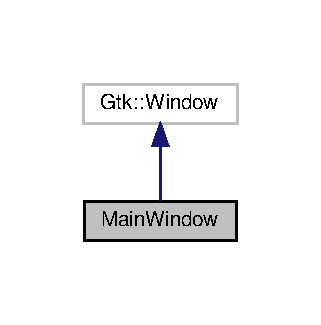
\includegraphics[width=154pt]{class_main_window__inherit__graph}
\end{center}
\end{figure}


Collaboration diagram for Main\+Window\+:\nopagebreak
\begin{figure}[H]
\begin{center}
\leavevmode
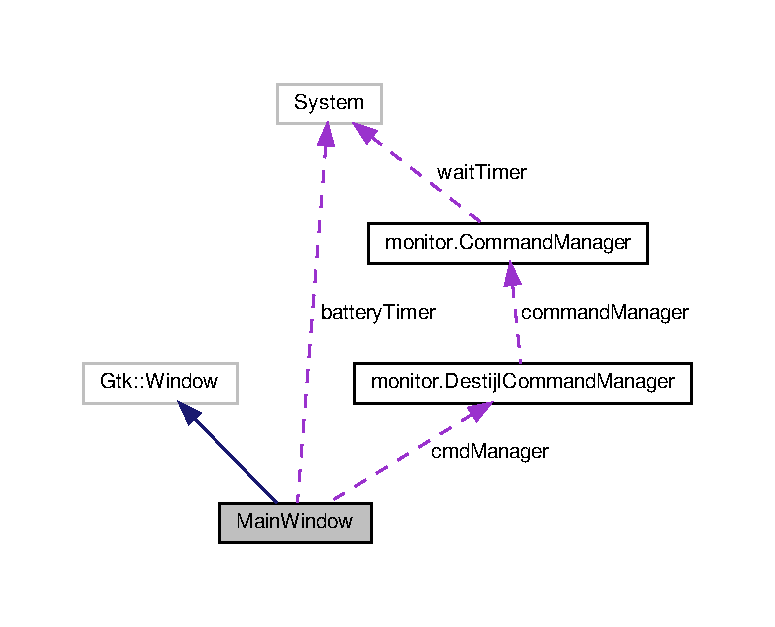
\includegraphics[width=350pt]{class_main_window__coll__graph}
\end{center}
\end{figure}
\subsection*{Public Member Functions}
\begin{DoxyCompactItemize}
\item 
\textbf{ Main\+Window} ()
\begin{DoxyCompactList}\small\item\em Initializes a new instance of the \doxyref{Main\+Window}{p.}{class_main_window} class. \end{DoxyCompactList}\item 
void \textbf{ Adjust\+Controls} ()
\begin{DoxyCompactList}\small\item\em Make some adjustement to controls, like disabling some controls \end{DoxyCompactList}\item 
void \textbf{ On\+Command\+Received\+Event} (string header, string data, byte[$\,$] buffer)
\begin{DoxyCompactList}\small\item\em Callback called when new message is received from server \end{DoxyCompactList}\end{DoxyCompactItemize}
\subsection*{Protected Member Functions}
\begin{DoxyCompactItemize}
\item 
void \textbf{ On\+Delete\+Event} (object sender, Delete\+Event\+Args a)
\begin{DoxyCompactList}\small\item\em Callback called when delete event is sent by window \end{DoxyCompactList}\item 
void \textbf{ On\+Quit\+Action\+Activated} (object sender, Event\+Args e)
\begin{DoxyCompactList}\small\item\em Callback called by \char`\"{}quit\char`\"{} menu \end{DoxyCompactList}\item 
void \textbf{ On\+Show\+Log\+Window\+Action\+Activated} (object sender, Event\+Args e)
\begin{DoxyCompactList}\small\item\em Callback called by \char`\"{}show log\char`\"{} menu \end{DoxyCompactList}\item 
void \textbf{ On\+Button\+Server\+Connection\+Clicked} (object sender, Event\+Args e)
\begin{DoxyCompactList}\small\item\em Callback called by \char`\"{}button\+Server\+Connection\char`\"{} button \end{DoxyCompactList}\item 
void \textbf{ On\+Button\+Robot\+Activation\+Clicked} (object sender, Event\+Args e)
\begin{DoxyCompactList}\small\item\em Callback called when \char`\"{}button\+Robotactivation\char`\"{} is clicked \end{DoxyCompactList}\item 
void \textbf{ On\+Button\+Mouv\+Clicked} (object sender, Event\+Args e)
\begin{DoxyCompactList}\small\item\em Callback called when user click on direction button \end{DoxyCompactList}\item 
void \textbf{ On\+Check\+Button\+Camera\+On\+Clicked} (object sender, Event\+Args e)
\begin{DoxyCompactList}\small\item\em Callback called when checkbutton for camera is clicked \end{DoxyCompactList}\item 
void \textbf{ On\+Check\+Button\+Robot\+Position\+Clicked} (object sender, Event\+Args e)
\begin{DoxyCompactList}\small\item\em Callback called when checkbutton robot position is clicked \end{DoxyCompactList}\item 
void \textbf{ On\+Drawing\+Area\+Camera\+Expose\+Event} (object o, Expose\+Event\+Args args)
\begin{DoxyCompactList}\small\item\em Callback called when drawingarea need refresh \end{DoxyCompactList}\item 
void \textbf{ Detect\+Arena} ()
\begin{DoxyCompactList}\small\item\em Show a popup asking user to tell if arena is correct or not \end{DoxyCompactList}\item 
void \textbf{ On\+Button\+Ask\+Arena\+Clicked} (object sender, Event\+Args e)
\begin{DoxyCompactList}\small\item\em Callback called when \char`\"{}detect Arena \char`\"{} button is clicked \end{DoxyCompactList}\end{DoxyCompactItemize}
\subsection*{Private Types}
\begin{DoxyCompactItemize}
\item 
enum \textbf{ System\+State} \{ \textbf{ System\+State.\+Not\+Connected}, 
\textbf{ System\+State.\+Server\+Connected}, 
\textbf{ System\+State.\+Robot\+Connected}
 \}\begin{DoxyCompactList}\small\item\em List of availble state for the application \end{DoxyCompactList}
\end{DoxyCompactItemize}
\subsection*{Private Member Functions}
\begin{DoxyCompactItemize}
\item 
void \textbf{ Change\+State} (\textbf{ System\+State} new\+State)
\begin{DoxyCompactList}\small\item\em Method used to change controls visibility (greyed or not) depending on current state \end{DoxyCompactList}\item 
void \textbf{ Message\+Popup} (Message\+Type type, Buttons\+Type buttons, string title, string message)
\begin{DoxyCompactList}\small\item\em Display a popup message window \end{DoxyCompactList}\item 
void \textbf{ On\+Battery\+Timer\+Elapsed} (object sender, System.\+Timers.\+Elapsed\+Event\+Args e)
\begin{DoxyCompactList}\small\item\em Callback called when battery timer expired \end{DoxyCompactList}\end{DoxyCompactItemize}
\subsection*{Private Attributes}
\begin{DoxyCompactItemize}
\item 
\textbf{ Destijl\+Command\+Manager} \textbf{ cmd\+Manager}
\begin{DoxyCompactList}\small\item\em Destijl command manager reference \end{DoxyCompactList}\item 
Pixbuf \textbf{ drawingarea\+Camera\+Pixbuf}
\begin{DoxyCompactList}\small\item\em Pixbuffer used for displaying image \end{DoxyCompactList}\item 
\textbf{ System\+State} \textbf{ system\+State} = \textbf{ System\+State.\+Not\+Connected}
\begin{DoxyCompactList}\small\item\em The state of the system. Can take a value from System\+State \end{DoxyCompactList}\item 
System.\+Timers.\+Timer \textbf{ battery\+Timer}
\begin{DoxyCompactList}\small\item\em Timer for battery request \end{DoxyCompactList}\end{DoxyCompactItemize}


\subsection{Detailed Description}
Main part of the program, behavior of main window 



Definition at line 32 of file Monitor\+U\+I.\+cs.



\subsection{Member Enumeration Documentation}
\mbox{\label{class_main_window_a7b18ca1f8f71faf272c9856aaf7b8e3d}} 
\index{Main\+Window@{Main\+Window}!System\+State@{System\+State}}
\index{System\+State@{System\+State}!Main\+Window@{Main\+Window}}
\subsubsection{System\+State}
{\footnotesize\ttfamily enum \textbf{ Main\+Window.\+System\+State}\hspace{0.3cm}{\ttfamily [strong]}, {\ttfamily [private]}}



List of availble state for the application 

\begin{DoxyEnumFields}{Enumerator}
\raisebox{\heightof{T}}[0pt][0pt]{\index{Not\+Connected@{Not\+Connected}!Main\+Window@{Main\+Window}}\index{Main\+Window@{Main\+Window}!Not\+Connected@{Not\+Connected}}}\mbox{\label{class_main_window_a7b18ca1f8f71faf272c9856aaf7b8e3da4075072d219e061ca0f3124f8fbef463}} 
Not\+Connected&\\
\hline

\raisebox{\heightof{T}}[0pt][0pt]{\index{Server\+Connected@{Server\+Connected}!Main\+Window@{Main\+Window}}\index{Main\+Window@{Main\+Window}!Server\+Connected@{Server\+Connected}}}\mbox{\label{class_main_window_a7b18ca1f8f71faf272c9856aaf7b8e3da911ba363fd1483b5b36fda7b0149cf76}} 
Server\+Connected&\\
\hline

\raisebox{\heightof{T}}[0pt][0pt]{\index{Robot\+Connected@{Robot\+Connected}!Main\+Window@{Main\+Window}}\index{Main\+Window@{Main\+Window}!Robot\+Connected@{Robot\+Connected}}}\mbox{\label{class_main_window_a7b18ca1f8f71faf272c9856aaf7b8e3da9761e78f9ae0d6f598d953b4d9e839e1}} 
Robot\+Connected&\\
\hline

\end{DoxyEnumFields}


Definition at line 47 of file Monitor\+U\+I.\+cs.



\subsection{Constructor \& Destructor Documentation}
\mbox{\label{class_main_window_af607d50e4d1b04d3c494661489283f45}} 
\index{Main\+Window@{Main\+Window}!Main\+Window@{Main\+Window}}
\index{Main\+Window@{Main\+Window}!Main\+Window@{Main\+Window}}
\subsubsection{Main\+Window()}
{\footnotesize\ttfamily Main\+Window.\+Main\+Window (\begin{DoxyParamCaption}{ }\end{DoxyParamCaption})}



Initializes a new instance of the \doxyref{Main\+Window}{p.}{class_main_window} class. 



Definition at line 67 of file Monitor\+U\+I.\+cs.



\subsection{Member Function Documentation}
\mbox{\label{class_main_window_a9a0f3d4cd871609f12d328af2f588664}} 
\index{Main\+Window@{Main\+Window}!Adjust\+Controls@{Adjust\+Controls}}
\index{Adjust\+Controls@{Adjust\+Controls}!Main\+Window@{Main\+Window}}
\subsubsection{Adjust\+Controls()}
{\footnotesize\ttfamily void Main\+Window.\+Adjust\+Controls (\begin{DoxyParamCaption}{ }\end{DoxyParamCaption})}



Make some adjustement to controls, like disabling some controls 



Definition at line 84 of file Monitor\+U\+I.\+cs.

\mbox{\label{class_main_window_aedc27cabbe1604313a452fcbf3ffe9f4}} 
\index{Main\+Window@{Main\+Window}!Change\+State@{Change\+State}}
\index{Change\+State@{Change\+State}!Main\+Window@{Main\+Window}}
\subsubsection{Change\+State()}
{\footnotesize\ttfamily void Main\+Window.\+Change\+State (\begin{DoxyParamCaption}\item[{\textbf{ System\+State}}]{new\+State }\end{DoxyParamCaption})\hspace{0.3cm}{\ttfamily [private]}}



Method used to change controls visibility (greyed or not) depending on current state 


\begin{DoxyParams}{Parameters}
{\em new\+State} & New state\\
\hline
\end{DoxyParams}


Definition at line 103 of file Monitor\+U\+I.\+cs.

\mbox{\label{class_main_window_a89c79ce9ca4114ca9c50f32dc080e9cd}} 
\index{Main\+Window@{Main\+Window}!Detect\+Arena@{Detect\+Arena}}
\index{Detect\+Arena@{Detect\+Arena}!Main\+Window@{Main\+Window}}
\subsubsection{Detect\+Arena()}
{\footnotesize\ttfamily void Main\+Window.\+Detect\+Arena (\begin{DoxyParamCaption}{ }\end{DoxyParamCaption})\hspace{0.3cm}{\ttfamily [protected]}}



Show a popup asking user to tell if arena is correct or not 



Definition at line 610 of file Monitor\+U\+I.\+cs.

\mbox{\label{class_main_window_afc4f923aaa481a93dddaff6303efb9e0}} 
\index{Main\+Window@{Main\+Window}!Message\+Popup@{Message\+Popup}}
\index{Message\+Popup@{Message\+Popup}!Main\+Window@{Main\+Window}}
\subsubsection{Message\+Popup()}
{\footnotesize\ttfamily void Main\+Window.\+Message\+Popup (\begin{DoxyParamCaption}\item[{Message\+Type}]{type,  }\item[{Buttons\+Type}]{buttons,  }\item[{string}]{title,  }\item[{string}]{message }\end{DoxyParamCaption})\hspace{0.3cm}{\ttfamily [private]}}



Display a popup message window 


\begin{DoxyParams}{Parameters}
{\em type} & Type of popup window (question, error, information,...)\\
\hline
{\em buttons} & Buttons available on popup window\\
\hline
{\em title} & Title of window\\
\hline
{\em message} & Message\\
\hline
\end{DoxyParams}


Definition at line 176 of file Monitor\+U\+I.\+cs.

\mbox{\label{class_main_window_af303b70c08cda04a76f6418f727c4891}} 
\index{Main\+Window@{Main\+Window}!On\+Battery\+Timer\+Elapsed@{On\+Battery\+Timer\+Elapsed}}
\index{On\+Battery\+Timer\+Elapsed@{On\+Battery\+Timer\+Elapsed}!Main\+Window@{Main\+Window}}
\subsubsection{On\+Battery\+Timer\+Elapsed()}
{\footnotesize\ttfamily void Main\+Window.\+On\+Battery\+Timer\+Elapsed (\begin{DoxyParamCaption}\item[{object}]{sender,  }\item[{System.\+Timers.\+Elapsed\+Event\+Args}]{e }\end{DoxyParamCaption})\hspace{0.3cm}{\ttfamily [private]}}



Callback called when battery timer expired 


\begin{DoxyParams}{Parameters}
{\em sender} & Sender object\\
\hline
{\em e} & Event\\
\hline
\end{DoxyParams}


Definition at line 457 of file Monitor\+U\+I.\+cs.

\mbox{\label{class_main_window_a31e299085d6286d680bd488c73fdff82}} 
\index{Main\+Window@{Main\+Window}!On\+Button\+Ask\+Arena\+Clicked@{On\+Button\+Ask\+Arena\+Clicked}}
\index{On\+Button\+Ask\+Arena\+Clicked@{On\+Button\+Ask\+Arena\+Clicked}!Main\+Window@{Main\+Window}}
\subsubsection{On\+Button\+Ask\+Arena\+Clicked()}
{\footnotesize\ttfamily void Main\+Window.\+On\+Button\+Ask\+Arena\+Clicked (\begin{DoxyParamCaption}\item[{object}]{sender,  }\item[{Event\+Args}]{e }\end{DoxyParamCaption})\hspace{0.3cm}{\ttfamily [protected]}}



Callback called when \char`\"{}detect Arena \char`\"{} button is clicked 


\begin{DoxyParams}{Parameters}
{\em sender} & Sender object\\
\hline
{\em e} & Event\\
\hline
\end{DoxyParams}


Definition at line 644 of file Monitor\+U\+I.\+cs.

\mbox{\label{class_main_window_a7f8d06747f887216ab8c941ad10cb48b}} 
\index{Main\+Window@{Main\+Window}!On\+Button\+Mouv\+Clicked@{On\+Button\+Mouv\+Clicked}}
\index{On\+Button\+Mouv\+Clicked@{On\+Button\+Mouv\+Clicked}!Main\+Window@{Main\+Window}}
\subsubsection{On\+Button\+Mouv\+Clicked()}
{\footnotesize\ttfamily void Main\+Window.\+On\+Button\+Mouv\+Clicked (\begin{DoxyParamCaption}\item[{object}]{sender,  }\item[{Event\+Args}]{e }\end{DoxyParamCaption})\hspace{0.3cm}{\ttfamily [protected]}}



Callback called when user click on direction button 


\begin{DoxyParams}{Parameters}
{\em sender} & Sender button\\
\hline
{\em e} & Event\\
\hline
\end{DoxyParams}


Definition at line 427 of file Monitor\+U\+I.\+cs.

\mbox{\label{class_main_window_a2b5e11a49a10b24c59bebb377cdfeae8}} 
\index{Main\+Window@{Main\+Window}!On\+Button\+Robot\+Activation\+Clicked@{On\+Button\+Robot\+Activation\+Clicked}}
\index{On\+Button\+Robot\+Activation\+Clicked@{On\+Button\+Robot\+Activation\+Clicked}!Main\+Window@{Main\+Window}}
\subsubsection{On\+Button\+Robot\+Activation\+Clicked()}
{\footnotesize\ttfamily void Main\+Window.\+On\+Button\+Robot\+Activation\+Clicked (\begin{DoxyParamCaption}\item[{object}]{sender,  }\item[{Event\+Args}]{e }\end{DoxyParamCaption})\hspace{0.3cm}{\ttfamily [protected]}}



Callback called when \char`\"{}button\+Robotactivation\char`\"{} is clicked 


\begin{DoxyParams}{Parameters}
{\em sender} & Sender object\\
\hline
{\em e} & Event\\
\hline
\end{DoxyParams}


Definition at line 363 of file Monitor\+U\+I.\+cs.

\mbox{\label{class_main_window_ac0acc6c3a63f405f14ec8e4d132a2661}} 
\index{Main\+Window@{Main\+Window}!On\+Button\+Server\+Connection\+Clicked@{On\+Button\+Server\+Connection\+Clicked}}
\index{On\+Button\+Server\+Connection\+Clicked@{On\+Button\+Server\+Connection\+Clicked}!Main\+Window@{Main\+Window}}
\subsubsection{On\+Button\+Server\+Connection\+Clicked()}
{\footnotesize\ttfamily void Main\+Window.\+On\+Button\+Server\+Connection\+Clicked (\begin{DoxyParamCaption}\item[{object}]{sender,  }\item[{Event\+Args}]{e }\end{DoxyParamCaption})\hspace{0.3cm}{\ttfamily [protected]}}



Callback called by \char`\"{}button\+Server\+Connection\char`\"{} button 


\begin{DoxyParams}{Parameters}
{\em sender} & Sender object\\
\hline
{\em e} & Event\\
\hline
\end{DoxyParams}


Definition at line 282 of file Monitor\+U\+I.\+cs.

\mbox{\label{class_main_window_af4b587cdd614d5bdb8d9158a1f59e4fa}} 
\index{Main\+Window@{Main\+Window}!On\+Check\+Button\+Camera\+On\+Clicked@{On\+Check\+Button\+Camera\+On\+Clicked}}
\index{On\+Check\+Button\+Camera\+On\+Clicked@{On\+Check\+Button\+Camera\+On\+Clicked}!Main\+Window@{Main\+Window}}
\subsubsection{On\+Check\+Button\+Camera\+On\+Clicked()}
{\footnotesize\ttfamily void Main\+Window.\+On\+Check\+Button\+Camera\+On\+Clicked (\begin{DoxyParamCaption}\item[{object}]{sender,  }\item[{Event\+Args}]{e }\end{DoxyParamCaption})\hspace{0.3cm}{\ttfamily [protected]}}



Callback called when checkbutton for camera is clicked 


\begin{DoxyParams}{Parameters}
{\em sender} & Sender object\\
\hline
{\em e} & Event\\
\hline
\end{DoxyParams}


Definition at line 501 of file Monitor\+U\+I.\+cs.

\mbox{\label{class_main_window_a20d07605619027d82a30552f294b128f}} 
\index{Main\+Window@{Main\+Window}!On\+Check\+Button\+Robot\+Position\+Clicked@{On\+Check\+Button\+Robot\+Position\+Clicked}}
\index{On\+Check\+Button\+Robot\+Position\+Clicked@{On\+Check\+Button\+Robot\+Position\+Clicked}!Main\+Window@{Main\+Window}}
\subsubsection{On\+Check\+Button\+Robot\+Position\+Clicked()}
{\footnotesize\ttfamily void Main\+Window.\+On\+Check\+Button\+Robot\+Position\+Clicked (\begin{DoxyParamCaption}\item[{object}]{sender,  }\item[{Event\+Args}]{e }\end{DoxyParamCaption})\hspace{0.3cm}{\ttfamily [protected]}}



Callback called when checkbutton robot position is clicked 


\begin{DoxyParams}{Parameters}
{\em sender} & Sender object\\
\hline
{\em e} & Event\\
\hline
\end{DoxyParams}


Definition at line 530 of file Monitor\+U\+I.\+cs.

\mbox{\label{class_main_window_a4b651f10b9079c128b9e36d15ad10211}} 
\index{Main\+Window@{Main\+Window}!On\+Command\+Received\+Event@{On\+Command\+Received\+Event}}
\index{On\+Command\+Received\+Event@{On\+Command\+Received\+Event}!Main\+Window@{Main\+Window}}
\subsubsection{On\+Command\+Received\+Event()}
{\footnotesize\ttfamily void Main\+Window.\+On\+Command\+Received\+Event (\begin{DoxyParamCaption}\item[{string}]{header,  }\item[{string}]{data,  }\item[{byte [$\,$]}]{buffer }\end{DoxyParamCaption})}



Callback called when new message is received from server 


\begin{DoxyParams}{Parameters}
{\em header} & Header of message\\
\hline
{\em data} & Data of message\\
\hline
{\em buffer} & Raw buffer corresponding of received message\\
\hline
\end{DoxyParams}


Definition at line 207 of file Monitor\+U\+I.\+cs.

\mbox{\label{class_main_window_a64bdcb29cebb58957790da1ee2733fe1}} 
\index{Main\+Window@{Main\+Window}!On\+Delete\+Event@{On\+Delete\+Event}}
\index{On\+Delete\+Event@{On\+Delete\+Event}!Main\+Window@{Main\+Window}}
\subsubsection{On\+Delete\+Event()}
{\footnotesize\ttfamily void Main\+Window.\+On\+Delete\+Event (\begin{DoxyParamCaption}\item[{object}]{sender,  }\item[{Delete\+Event\+Args}]{a }\end{DoxyParamCaption})\hspace{0.3cm}{\ttfamily [protected]}}



Callback called when delete event is sent by window 


\begin{DoxyParams}{Parameters}
{\em sender} & Sender object\\
\hline
{\em a} & Not really sure of what it is...\\
\hline
\end{DoxyParams}


Definition at line 192 of file Monitor\+U\+I.\+cs.

\mbox{\label{class_main_window_afe4b0001f191554aed5d9b65208a06f5}} 
\index{Main\+Window@{Main\+Window}!On\+Drawing\+Area\+Camera\+Expose\+Event@{On\+Drawing\+Area\+Camera\+Expose\+Event}}
\index{On\+Drawing\+Area\+Camera\+Expose\+Event@{On\+Drawing\+Area\+Camera\+Expose\+Event}!Main\+Window@{Main\+Window}}
\subsubsection{On\+Drawing\+Area\+Camera\+Expose\+Event()}
{\footnotesize\ttfamily void Main\+Window.\+On\+Drawing\+Area\+Camera\+Expose\+Event (\begin{DoxyParamCaption}\item[{object}]{o,  }\item[{Expose\+Event\+Args}]{args }\end{DoxyParamCaption})\hspace{0.3cm}{\ttfamily [protected]}}



Callback called when drawingarea need refresh 


\begin{DoxyParams}{Parameters}
{\em o} & Sender object\\
\hline
{\em args} & Expose arguments\\
\hline
\end{DoxyParams}


Definition at line 560 of file Monitor\+U\+I.\+cs.

\mbox{\label{class_main_window_ab54b643c364b46a150f6f993267bb709}} 
\index{Main\+Window@{Main\+Window}!On\+Quit\+Action\+Activated@{On\+Quit\+Action\+Activated}}
\index{On\+Quit\+Action\+Activated@{On\+Quit\+Action\+Activated}!Main\+Window@{Main\+Window}}
\subsubsection{On\+Quit\+Action\+Activated()}
{\footnotesize\ttfamily void Main\+Window.\+On\+Quit\+Action\+Activated (\begin{DoxyParamCaption}\item[{object}]{sender,  }\item[{Event\+Args}]{e }\end{DoxyParamCaption})\hspace{0.3cm}{\ttfamily [protected]}}



Callback called by \char`\"{}quit\char`\"{} menu 


\begin{DoxyParams}{Parameters}
{\em sender} & Sender object\\
\hline
{\em e} & Event\\
\hline
\end{DoxyParams}


Definition at line 257 of file Monitor\+U\+I.\+cs.

\mbox{\label{class_main_window_a87132738a6ca496303940d56e091bdc7}} 
\index{Main\+Window@{Main\+Window}!On\+Show\+Log\+Window\+Action\+Activated@{On\+Show\+Log\+Window\+Action\+Activated}}
\index{On\+Show\+Log\+Window\+Action\+Activated@{On\+Show\+Log\+Window\+Action\+Activated}!Main\+Window@{Main\+Window}}
\subsubsection{On\+Show\+Log\+Window\+Action\+Activated()}
{\footnotesize\ttfamily void Main\+Window.\+On\+Show\+Log\+Window\+Action\+Activated (\begin{DoxyParamCaption}\item[{object}]{sender,  }\item[{Event\+Args}]{e }\end{DoxyParamCaption})\hspace{0.3cm}{\ttfamily [protected]}}



Callback called by \char`\"{}show log\char`\"{} menu 


\begin{DoxyParams}{Parameters}
{\em sender} & Sender object\\
\hline
{\em e} & Event\\
\hline
\end{DoxyParams}


Definition at line 270 of file Monitor\+U\+I.\+cs.



\subsection{Member Data Documentation}
\mbox{\label{class_main_window_a57f0325d8b8a63be586001b9a469d9ae}} 
\index{Main\+Window@{Main\+Window}!battery\+Timer@{battery\+Timer}}
\index{battery\+Timer@{battery\+Timer}!Main\+Window@{Main\+Window}}
\subsubsection{battery\+Timer}
{\footnotesize\ttfamily System.\+Timers.\+Timer Main\+Window.\+battery\+Timer\hspace{0.3cm}{\ttfamily [private]}}



Timer for battery request 



Definition at line 62 of file Monitor\+U\+I.\+cs.

\mbox{\label{class_main_window_a0b60450970b8a6fb6e016d5c0728e474}} 
\index{Main\+Window@{Main\+Window}!cmd\+Manager@{cmd\+Manager}}
\index{cmd\+Manager@{cmd\+Manager}!Main\+Window@{Main\+Window}}
\subsubsection{cmd\+Manager}
{\footnotesize\ttfamily \textbf{ Destijl\+Command\+Manager} Main\+Window.\+cmd\+Manager\hspace{0.3cm}{\ttfamily [private]}}



Destijl command manager reference 



Definition at line 37 of file Monitor\+U\+I.\+cs.

\mbox{\label{class_main_window_a41581e449b18e87acbdff5baa12c2050}} 
\index{Main\+Window@{Main\+Window}!drawingarea\+Camera\+Pixbuf@{drawingarea\+Camera\+Pixbuf}}
\index{drawingarea\+Camera\+Pixbuf@{drawingarea\+Camera\+Pixbuf}!Main\+Window@{Main\+Window}}
\subsubsection{drawingarea\+Camera\+Pixbuf}
{\footnotesize\ttfamily Pixbuf Main\+Window.\+drawingarea\+Camera\+Pixbuf\hspace{0.3cm}{\ttfamily [private]}}



Pixbuffer used for displaying image 



Definition at line 42 of file Monitor\+U\+I.\+cs.

\mbox{\label{class_main_window_a105025ee1bdfac188f1ce640d593550d}} 
\index{Main\+Window@{Main\+Window}!system\+State@{system\+State}}
\index{system\+State@{system\+State}!Main\+Window@{Main\+Window}}
\subsubsection{system\+State}
{\footnotesize\ttfamily \textbf{ System\+State} Main\+Window.\+system\+State = \textbf{ System\+State.\+Not\+Connected}\hspace{0.3cm}{\ttfamily [private]}}



The state of the system. Can take a value from System\+State 



Definition at line 57 of file Monitor\+U\+I.\+cs.



The documentation for this class was generated from the following file\+:\begin{DoxyCompactItemize}
\item 
\textbf{ Monitor\+U\+I.\+cs}\end{DoxyCompactItemize}

\section{monitor.\+Robot\+Command\+List Class Reference}
\label{classmonitor_1_1_robot_command_list}\index{monitor.\+Robot\+Command\+List@{monitor.\+Robot\+Command\+List}}


Commands used for robot messages  


\subsection*{Public Attributes}
\begin{DoxyCompactItemize}
\item 
const string \textbf{ Robot\+Ping} = \char`\"{}p\char`\"{}
\item 
const string \textbf{ Robot\+Reset} = \char`\"{}r\char`\"{}
\item 
const string \textbf{ Robot\+Start\+Without\+Watchdog} = \char`\"{}u\char`\"{}
\item 
const string \textbf{ Robot\+Start\+With\+Watchdog} = \char`\"{}W\char`\"{}
\item 
const string \textbf{ Robot\+Get\+Battery} = \char`\"{}v\char`\"{}
\item 
const string \textbf{ Robot\+Get\+Busy\+State} = \char`\"{}b\char`\"{}
\item 
const string \textbf{ Robot\+Move} = \char`\"{}M\char`\"{}
\item 
const string \textbf{ Robot\+Turn} = \char`\"{}T\char`\"{}
\item 
const string \textbf{ Robot\+Get\+Version} = \char`\"{}V\char`\"{}
\item 
const string \textbf{ Robot\+Power\+Off} = \char`\"{}z\char`\"{}
\end{DoxyCompactItemize}


\subsection{Detailed Description}
Commands used for robot messages 



Definition at line 59 of file Destijl\+Command\+Manager.\+cs.



\subsection{Member Data Documentation}
\mbox{\label{classmonitor_1_1_robot_command_list_a374eb526d14b8499e47b065230afeed0}} 
\index{monitor\+::\+Robot\+Command\+List@{monitor\+::\+Robot\+Command\+List}!Robot\+Get\+Battery@{Robot\+Get\+Battery}}
\index{Robot\+Get\+Battery@{Robot\+Get\+Battery}!monitor\+::\+Robot\+Command\+List@{monitor\+::\+Robot\+Command\+List}}
\subsubsection{Robot\+Get\+Battery}
{\footnotesize\ttfamily const string monitor.\+Robot\+Command\+List.\+Robot\+Get\+Battery = \char`\"{}v\char`\"{}}



Definition at line 65 of file Destijl\+Command\+Manager.\+cs.

\mbox{\label{classmonitor_1_1_robot_command_list_a52a901f4e013dc33ff491c5fcda76860}} 
\index{monitor\+::\+Robot\+Command\+List@{monitor\+::\+Robot\+Command\+List}!Robot\+Get\+Busy\+State@{Robot\+Get\+Busy\+State}}
\index{Robot\+Get\+Busy\+State@{Robot\+Get\+Busy\+State}!monitor\+::\+Robot\+Command\+List@{monitor\+::\+Robot\+Command\+List}}
\subsubsection{Robot\+Get\+Busy\+State}
{\footnotesize\ttfamily const string monitor.\+Robot\+Command\+List.\+Robot\+Get\+Busy\+State = \char`\"{}b\char`\"{}}



Definition at line 66 of file Destijl\+Command\+Manager.\+cs.

\mbox{\label{classmonitor_1_1_robot_command_list_a9a845beb5c040e4813f03cee7cd1cb71}} 
\index{monitor\+::\+Robot\+Command\+List@{monitor\+::\+Robot\+Command\+List}!Robot\+Get\+Version@{Robot\+Get\+Version}}
\index{Robot\+Get\+Version@{Robot\+Get\+Version}!monitor\+::\+Robot\+Command\+List@{monitor\+::\+Robot\+Command\+List}}
\subsubsection{Robot\+Get\+Version}
{\footnotesize\ttfamily const string monitor.\+Robot\+Command\+List.\+Robot\+Get\+Version = \char`\"{}V\char`\"{}}



Definition at line 69 of file Destijl\+Command\+Manager.\+cs.

\mbox{\label{classmonitor_1_1_robot_command_list_af7017bac04f1976fe1c37e8ec77bcbce}} 
\index{monitor\+::\+Robot\+Command\+List@{monitor\+::\+Robot\+Command\+List}!Robot\+Move@{Robot\+Move}}
\index{Robot\+Move@{Robot\+Move}!monitor\+::\+Robot\+Command\+List@{monitor\+::\+Robot\+Command\+List}}
\subsubsection{Robot\+Move}
{\footnotesize\ttfamily const string monitor.\+Robot\+Command\+List.\+Robot\+Move = \char`\"{}M\char`\"{}}



Definition at line 67 of file Destijl\+Command\+Manager.\+cs.

\mbox{\label{classmonitor_1_1_robot_command_list_a93de788c0d7ed40caaa2e3912a429831}} 
\index{monitor\+::\+Robot\+Command\+List@{monitor\+::\+Robot\+Command\+List}!Robot\+Ping@{Robot\+Ping}}
\index{Robot\+Ping@{Robot\+Ping}!monitor\+::\+Robot\+Command\+List@{monitor\+::\+Robot\+Command\+List}}
\subsubsection{Robot\+Ping}
{\footnotesize\ttfamily const string monitor.\+Robot\+Command\+List.\+Robot\+Ping = \char`\"{}p\char`\"{}}



Definition at line 61 of file Destijl\+Command\+Manager.\+cs.

\mbox{\label{classmonitor_1_1_robot_command_list_a2e9616c1b75719c208902e595b79cc48}} 
\index{monitor\+::\+Robot\+Command\+List@{monitor\+::\+Robot\+Command\+List}!Robot\+Power\+Off@{Robot\+Power\+Off}}
\index{Robot\+Power\+Off@{Robot\+Power\+Off}!monitor\+::\+Robot\+Command\+List@{monitor\+::\+Robot\+Command\+List}}
\subsubsection{Robot\+Power\+Off}
{\footnotesize\ttfamily const string monitor.\+Robot\+Command\+List.\+Robot\+Power\+Off = \char`\"{}z\char`\"{}}



Definition at line 70 of file Destijl\+Command\+Manager.\+cs.

\mbox{\label{classmonitor_1_1_robot_command_list_a9ef80510dfe9ca241af290b003766526}} 
\index{monitor\+::\+Robot\+Command\+List@{monitor\+::\+Robot\+Command\+List}!Robot\+Reset@{Robot\+Reset}}
\index{Robot\+Reset@{Robot\+Reset}!monitor\+::\+Robot\+Command\+List@{monitor\+::\+Robot\+Command\+List}}
\subsubsection{Robot\+Reset}
{\footnotesize\ttfamily const string monitor.\+Robot\+Command\+List.\+Robot\+Reset = \char`\"{}r\char`\"{}}



Definition at line 62 of file Destijl\+Command\+Manager.\+cs.

\mbox{\label{classmonitor_1_1_robot_command_list_a92acfe998bb9d265dd1f34f68f718386}} 
\index{monitor\+::\+Robot\+Command\+List@{monitor\+::\+Robot\+Command\+List}!Robot\+Start\+Without\+Watchdog@{Robot\+Start\+Without\+Watchdog}}
\index{Robot\+Start\+Without\+Watchdog@{Robot\+Start\+Without\+Watchdog}!monitor\+::\+Robot\+Command\+List@{monitor\+::\+Robot\+Command\+List}}
\subsubsection{Robot\+Start\+Without\+Watchdog}
{\footnotesize\ttfamily const string monitor.\+Robot\+Command\+List.\+Robot\+Start\+Without\+Watchdog = \char`\"{}u\char`\"{}}



Definition at line 63 of file Destijl\+Command\+Manager.\+cs.

\mbox{\label{classmonitor_1_1_robot_command_list_aafa5d0e5fec3afe6586cca8b88d45c85}} 
\index{monitor\+::\+Robot\+Command\+List@{monitor\+::\+Robot\+Command\+List}!Robot\+Start\+With\+Watchdog@{Robot\+Start\+With\+Watchdog}}
\index{Robot\+Start\+With\+Watchdog@{Robot\+Start\+With\+Watchdog}!monitor\+::\+Robot\+Command\+List@{monitor\+::\+Robot\+Command\+List}}
\subsubsection{Robot\+Start\+With\+Watchdog}
{\footnotesize\ttfamily const string monitor.\+Robot\+Command\+List.\+Robot\+Start\+With\+Watchdog = \char`\"{}W\char`\"{}}



Definition at line 64 of file Destijl\+Command\+Manager.\+cs.

\mbox{\label{classmonitor_1_1_robot_command_list_a2b88fc42fba8229f163e03e7252a77e6}} 
\index{monitor\+::\+Robot\+Command\+List@{monitor\+::\+Robot\+Command\+List}!Robot\+Turn@{Robot\+Turn}}
\index{Robot\+Turn@{Robot\+Turn}!monitor\+::\+Robot\+Command\+List@{monitor\+::\+Robot\+Command\+List}}
\subsubsection{Robot\+Turn}
{\footnotesize\ttfamily const string monitor.\+Robot\+Command\+List.\+Robot\+Turn = \char`\"{}T\char`\"{}}



Definition at line 68 of file Destijl\+Command\+Manager.\+cs.



The documentation for this class was generated from the following file\+:\begin{DoxyCompactItemize}
\item 
\textbf{ Destijl\+Command\+Manager.\+cs}\end{DoxyCompactItemize}

\chapter{File Documentation}
\section{Client.\+cs File Reference}
\label{_client_8cs}\index{Client.\+cs@{Client.\+cs}}
\subsection*{Classes}
\begin{DoxyCompactItemize}
\item 
class \textbf{ monitor.\+Client}
\begin{DoxyCompactList}\small\item\em Static class for T\+CP client \end{DoxyCompactList}\end{DoxyCompactItemize}
\subsection*{Namespaces}
\begin{DoxyCompactItemize}
\item 
namespace \textbf{ monitor}
\end{DoxyCompactItemize}

\section{Command\+Manager.\+cs File Reference}
\label{_command_manager_8cs}\index{Command\+Manager.\+cs@{Command\+Manager.\+cs}}
\subsection*{Classes}
\begin{DoxyCompactItemize}
\item 
class \textbf{ monitor.\+Command\+Manager}
\begin{DoxyCompactList}\small\item\em Command Manager. Use for timeout managment during reception of data Used as intermediate layer between T\+CP client class (\doxyref{Client}{p.}{classmonitor_1_1_client}) and application level managment of command and answers \end{DoxyCompactList}\end{DoxyCompactItemize}
\subsection*{Namespaces}
\begin{DoxyCompactItemize}
\item 
namespace \textbf{ monitor}
\end{DoxyCompactItemize}

\section{Destijl\+Command\+Manager.\+cs File Reference}
\label{_destijl_command_manager_8cs}\index{Destijl\+Command\+Manager.\+cs@{Destijl\+Command\+Manager.\+cs}}
\subsection*{Classes}
\begin{DoxyCompactItemize}
\item 
class \textbf{ monitor.\+Destijl\+Command\+List}
\item 
class \textbf{ monitor.\+Robot\+Command\+List}
\item 
class \textbf{ monitor.\+Destijl\+Command\+Manager}
\end{DoxyCompactItemize}
\subsection*{Namespaces}
\begin{DoxyCompactItemize}
\item 
namespace \textbf{ monitor}
\end{DoxyCompactItemize}

\section{Monitor\+U\+I.\+cs File Reference}
\label{_monitor_u_i_8cs}\index{Monitor\+U\+I.\+cs@{Monitor\+U\+I.\+cs}}
\subsection*{Classes}
\begin{DoxyCompactItemize}
\item 
class \textbf{ Main\+Window}
\begin{DoxyCompactList}\small\item\em Main window. \end{DoxyCompactList}\end{DoxyCompactItemize}

\section{Program.\+cs File Reference}
\label{_program_8cs}\index{Program.\+cs@{Program.\+cs}}
\subsection*{Classes}
\begin{DoxyCompactItemize}
\item 
class \textbf{ monitor.\+Main\+Class}
\end{DoxyCompactItemize}
\subsection*{Namespaces}
\begin{DoxyCompactItemize}
\item 
namespace \textbf{ monitor}
\end{DoxyCompactItemize}

%--- End generated contents ---

% Index
\backmatter
\newpage
\phantomsection
\clearemptydoublepage
\addcontentsline{toc}{chapter}{Index}
\printindex

\end{document}
